%%%%%%%%%%%%%%%%%%%%%%%%%%%%%%%%%%%%%%%%%%%%%%%%%%%%%%%%%%%%%%%%%%%%%%%%%
%                           Marco Conceptual                               %
%%%%%%%%%%%%%%%%%%%%%%%%%%%%%%%%%%%%%%%%%%%%%%%%%%%%%%%%%%%%%%%%%%%%%%%%%

\chapter{Marco conceptual}\label{chapter2}

Dado que este trabajo terminal emplea conceptos de diversas áreas de la Ingeniería en Sistemas Computacionales, resulta fundamental abordar una serie de definiciones previas que permitirán un mejor entendimiento del documento.


\section{Sistema Fotovoltaico}
Un sistema fotovoltaico es un conjunto de dispositivos que aprovechan la energía producida por el Sol y la convierten en energía eléctrica \citep{MarcoTeorico1}. Un sistema fotovoltaico puede ser “interconectado” para residencias o negocios con acceso a la red eléctrica. 

\paragraph{}
Con este sistema la energía generada se inyecta a la red eléctrica, disminuyendo así el consumo de energía de la compañía de luz. La otra opción es un sistema “isla” que permite el suministro de energía eléctrica en lugares inaccesibles para la red eléctrica. Estos sistemas son usados principalmente en casas de campo o en antenas de telecomunicación.
\paragraph{}
La particularidad de la corriente eléctrica generada por el efecto fotovoltaico es que esta corriente es continua, por lo cual el inversor transforma la corriente continua en alterna al estándar de la Norma Oficial Mexicana NOM-001-SEDE-2012 de Instalaciones Eléctricas (127 Volts a 60 Hertz) \citep{NORMA-Electrica} para ser alimentada a la red eléctrica, en la figura 2.1 se muestra la típica configuración de un sistema fotovoltaico:

\begin{figure}[H]
	\centering
	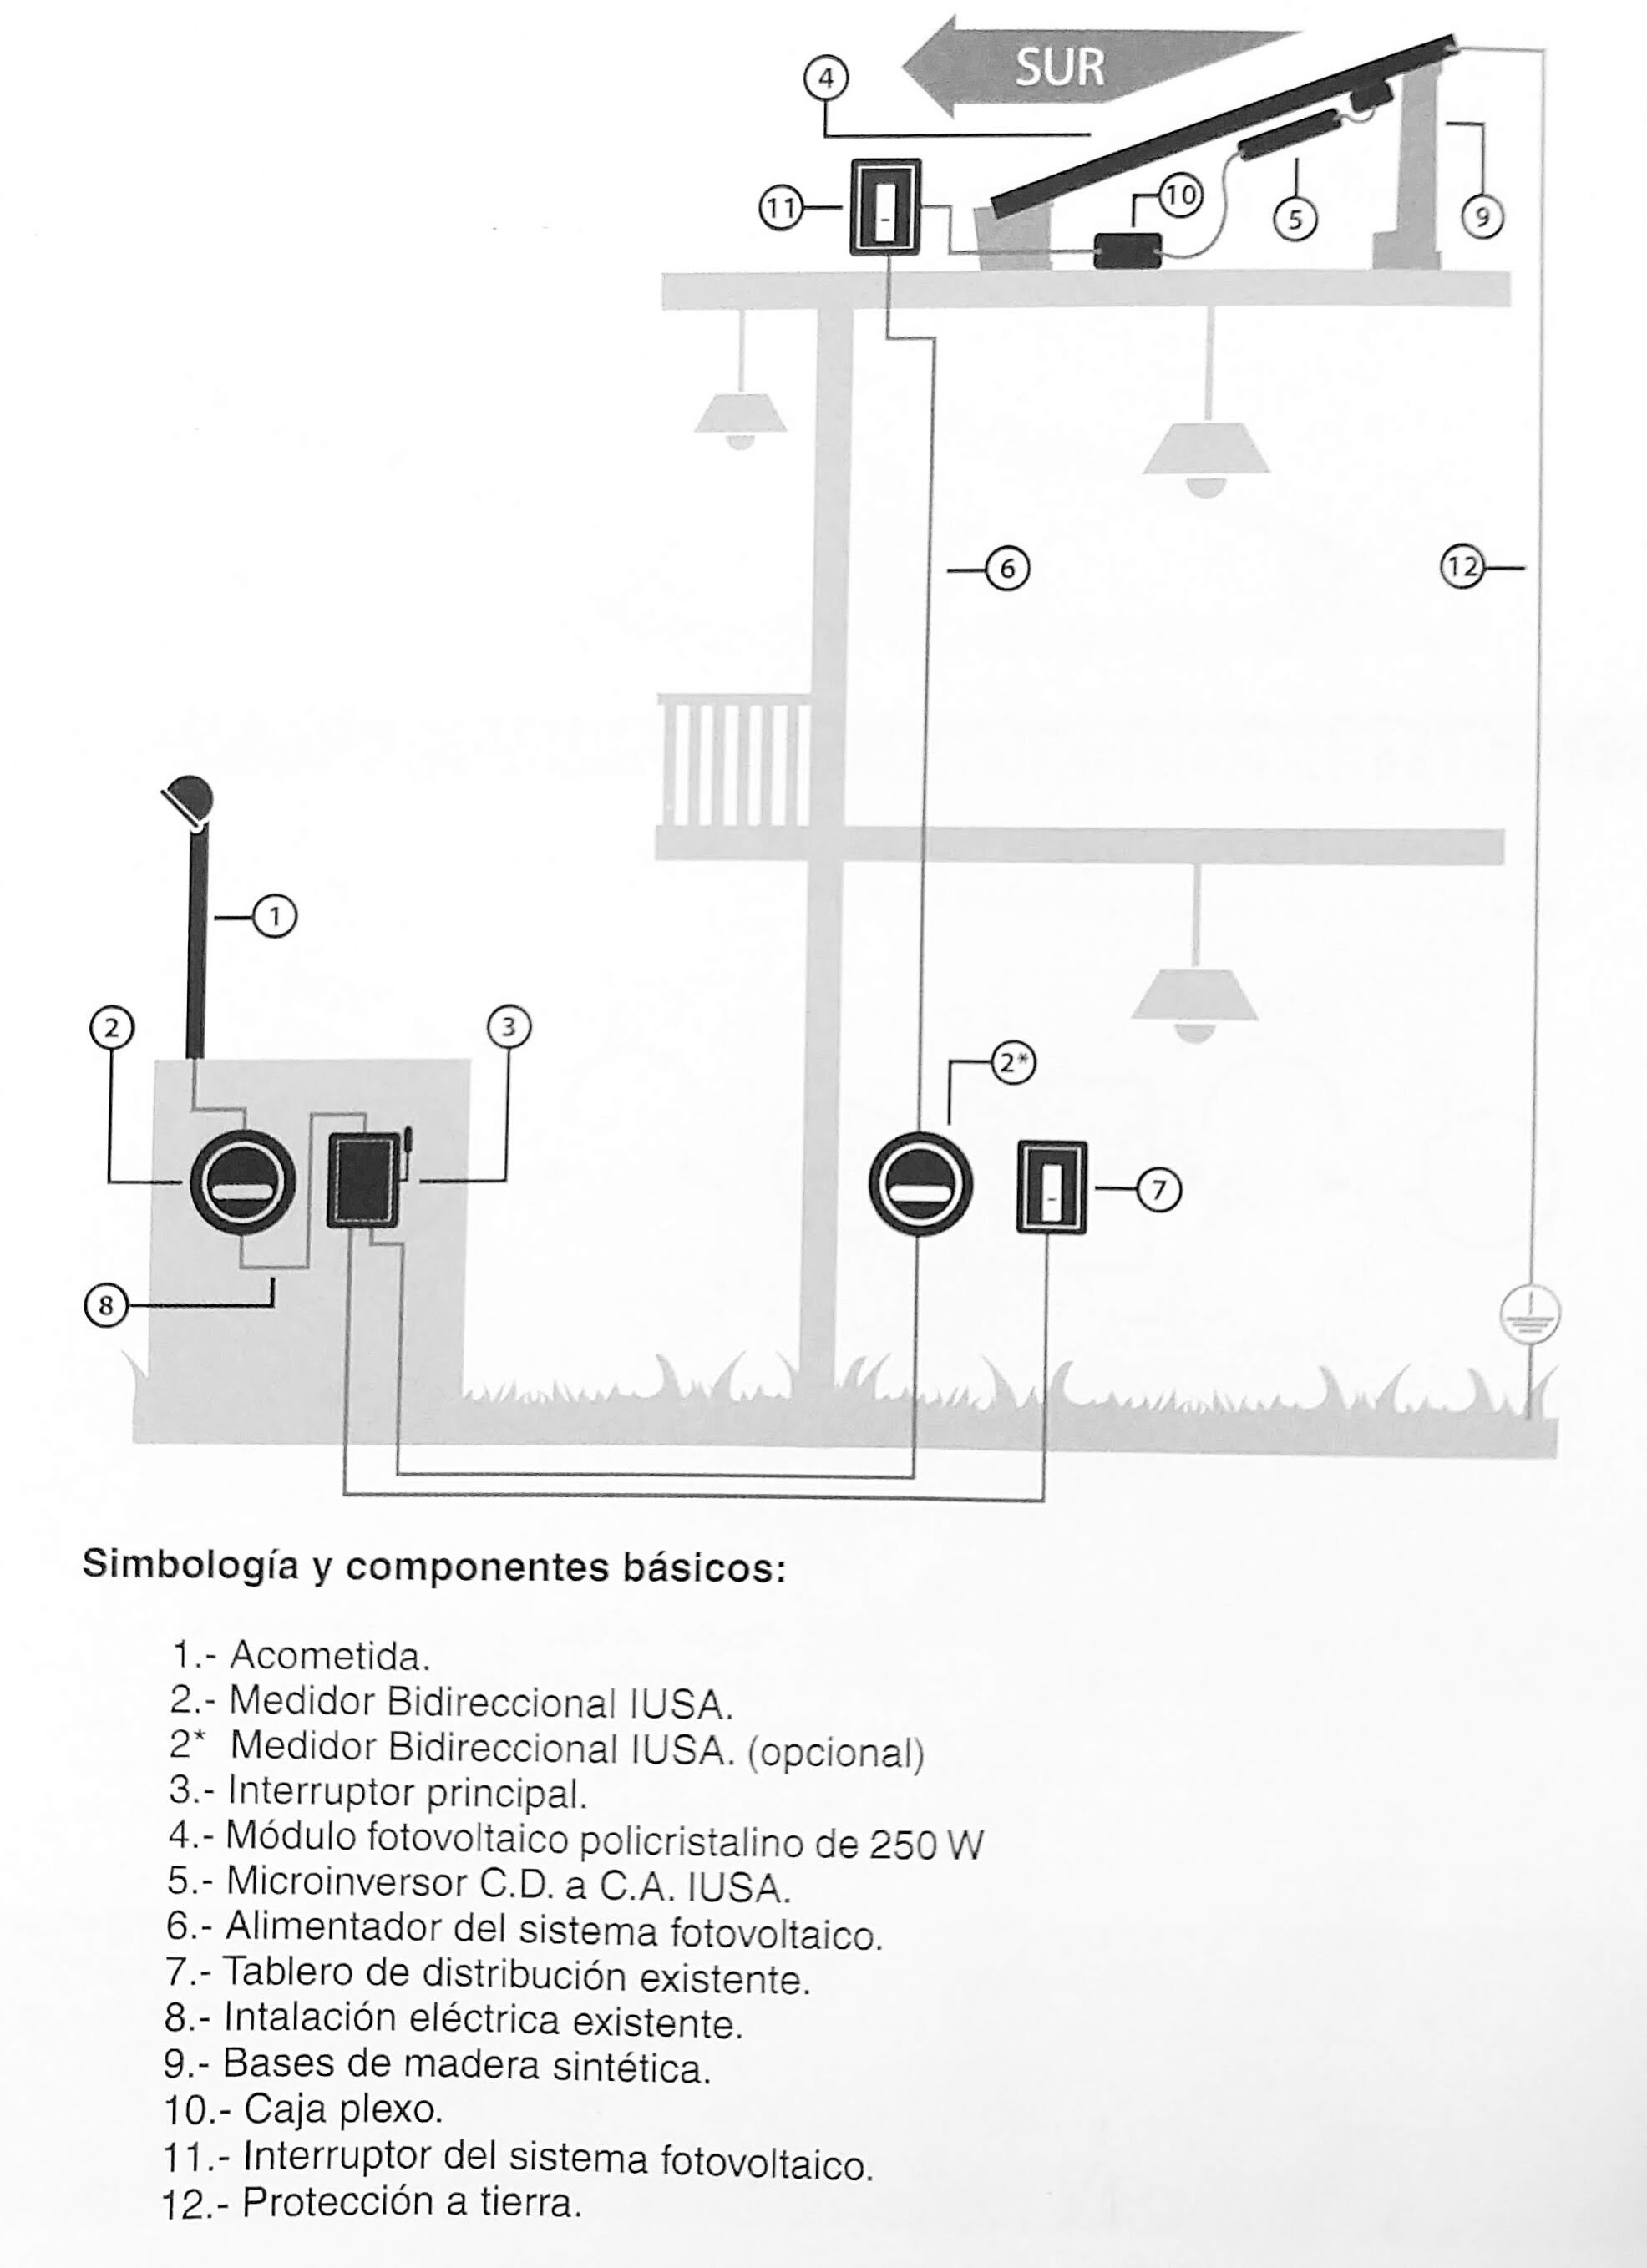
\includegraphics[scale=.1]{Capitulo2/images/sistema-fotovoltaico.jpg}
	\caption{Sistema Fotovoltaico Propuesto por el Fabricante IUSA}
	\label{fig:diagrama_dispensador}
\end{figure}

\paragraph{Ley para el Aprovechamiento de Energías Renovables}
Las fuentes de energía renovables y las tecnologías limpias para generar electricidad se convierten en parte medular de un proceso de transición energética con la publicación de la
Ley para el Aprovechamiento de Energías Renovables y el Financiamiento de la Transición
Energética el 28 de noviembre de 2008, así como el Reglamento de la citada Ley el 2 de septiembre de 2009, además se resalta la importancia de establecer un programa de normalización en la
materia, que provea de las regulaciones y normas necesarias \citep{LeyAprovechamiento}.



\paragraph{NMX-J-643/1}
Esta Norma Mexicana establece los procedimientos para la medición de las
características corriente-tensión de dispositivos fotovoltaicos,
con luz solar natural o con un simulador solar. Estos
procedimientos son aplicables a una celda solar fotovoltaica
individual o un conjunto ensamblado de celdas solares
fotovoltaicas que forman un módulo fotovoltaico \citep{NMX-J-643/1}.

\paragraph{NMX-J-618/1}
Establece los requisitos de construcción para módulos fotovoltaicos (FV), con la finalidad de proporcionar operación mecánica y eléctrica segura, durante su vida útil. Se mencionan recomendaciones específicas para la prevención de choque eléctrico, riesgo de incendio y lesiones personales, que se originan por esfuerzos mecánicos y ambientales \citep{NMX-J-618/1}.

\paragraph{Contrato de interconexión para paneles solares}

Una vez que instalas tu sistema solar en tu casa o negocio es necesario realizar un contrato de interconexión con CFE. La finalidad del contrato de interconexión es que CFE reconozca tu sistema solar y te acredite los kWh generados y enviados a la red eléctrica. CFE no te pagará de forma directa por la energía generada por tu sistema solar fotovoltaico. En su lugar, te darán un medidor bidireccional que registra tanto la energía consumida en tu casa habitación como la energía generada por tu sistema solar \citep{ContratoSolar}.
\paragraph{}
Realizar un contrato de interconexión en el cual CFE te autoriza utilizar la red eléctrica y darte crédito por los kWh generados por tu sistema solar suena complicado y hasta improbable. Sin embargo, CFE ha realizado un serie de cambios administrativos y realizar el contrato de interconexión resulta muy sencillo. A continuación, explicamos algunos de los requisitos para concretar dicho contrato.
\paragraph{}
El primero paso es llenar la solicitud de conexión, la información solicitada incluye la dirección donde se instala el sistema solar, la tarifa de consumo eléctrica actual y el RPU que es el número de cliente del contrato actual. También piden información más técnica en referencia al sistema solar tales como tamaño del sistema, la marcas y capacidades de los equipos, etc.
\paragraph{}
El contrato tiene costo que incluye el cambio de tu medidor actual a un medidor bidireccional. Es importante destacar que este no es el costo del medidor, ni tampoco se está comprando el medidor. Este le pertenece siempre a CFE y el monto a pagar solo incluye la programación e instalación del mismo.
\paragraph{}
Unos de los requisitos más importantes de la instalación que cabe mencionar aquí es que la conexión del sistema solar debe hacerse a baja tensión. Además, en el caso de instalaciones residenciales, el sistema fotovoltaico no puede exceder los 10kW de potencia pico. Para servicio de uso general o sistemas comerciales, el sistema solar puede ser de hasta 30kW de potencia.
\paragraph{}

\paragraph{Panel fotovoltaico}
Los paneles fotovoltaicos, llamados comúnmente paneles solares, están formados por un conjunto de células fotovoltaicas que producen electricidad a partir de la luz que incide sobre ellos mediante el efecto fotoeléctrico.
\paragraph{}
En la figura 2.2 se ilustra el efecto que consiste en la capacidad de algunos materiales (llamados semiconductores) de captar una parte de la energía de la luz para generar corriente eléctrica. En concreto, son los fotones los cuales transmiten una parte de su energía a ciertos electrones del material semiconductor. Estos electrones se “excitan”, y empiezan a fluir debido a la diferencia de potencial creando así corriente eléctrica \citep{MarcoTeorico2}.

\begin{figure}[H]
	\centering
	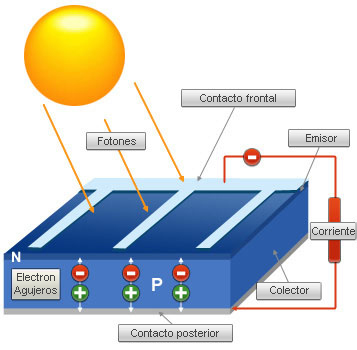
\includegraphics[scale=.50]{Capitulo2/images/celula-fotovoltaica.jpg}
	\caption{Efecto Fotoeléctrico}
	\label{fig:diagrama_dispensador}
\end{figure}

\paragraph{}
Los paneles fotovoltaicos se clasifican en función del tipo de célula que los forman, hay células cristalinas y amorfas, las células cristalinas se dividen de la siguiente forma :

\begin{itemize}
	\item Monocristalinas: se componen de secciones de un único cristal de silicio reconocibles por su forma circular u octogonal.
	\item Policristalinas: cuando están formadas por pequeñas partículas cristalizadas.
\end{itemize}

\begin{figure}[H]
	\centering
	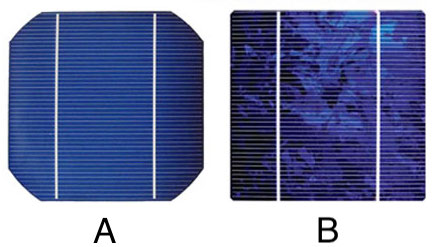
\includegraphics[scale=.50]{Capitulo2/images/tipospaneles.jpg}
	\caption{A: célula monocristalina ; B: célula policristalina}
	\label{fig:diagrama_dispensador}
\end{figure}

El costo de los paneles fotovoltaicos se ha reducido de forma constante desde que se fabricaron las primeras células solares comerciales y su costo promedio de generación eléctrica ya es competitivo con las fuentes de energía convencionales en un creciente número de regiones geográficas.
Los paneles fotovoltaicos pueden generar una gran cantidad de energía ya que en un día soleado, el Sol puede irradiar alrededor de 1kw por metro cuadrado a la superficie de la tierra, que sumado a la eficacia de estos paneles puede generar entre 120 y 250 w de manera constante por metro cuadrado, siempre dependiendo del tipo de panel y de su nivel de eficiencia.

\paragraph{Módulo Fotovoltaico 250W Policristalino IUSA}
Módulo fotovoltaico al estándar de las normas mexicanas NMX-J-643 y NMX-J-618, se muestra en la siguiente imagen, con 60 celdas en silicio policristalino, vidrio templado anti reflejante de 3.2 mm, caja de conexión IP67 con 3 diodos bypass y conectores compatibles con MC4.
Tiene una potencia máxima de 250W y un voltaje máximo de 30.6V, con una eficiencia del 15.1\% y temperatura de operación entre los -40ºC a los 85ºC. \citep{MarcoTeorico3}.

\begin{figure}[H]
	\centering
	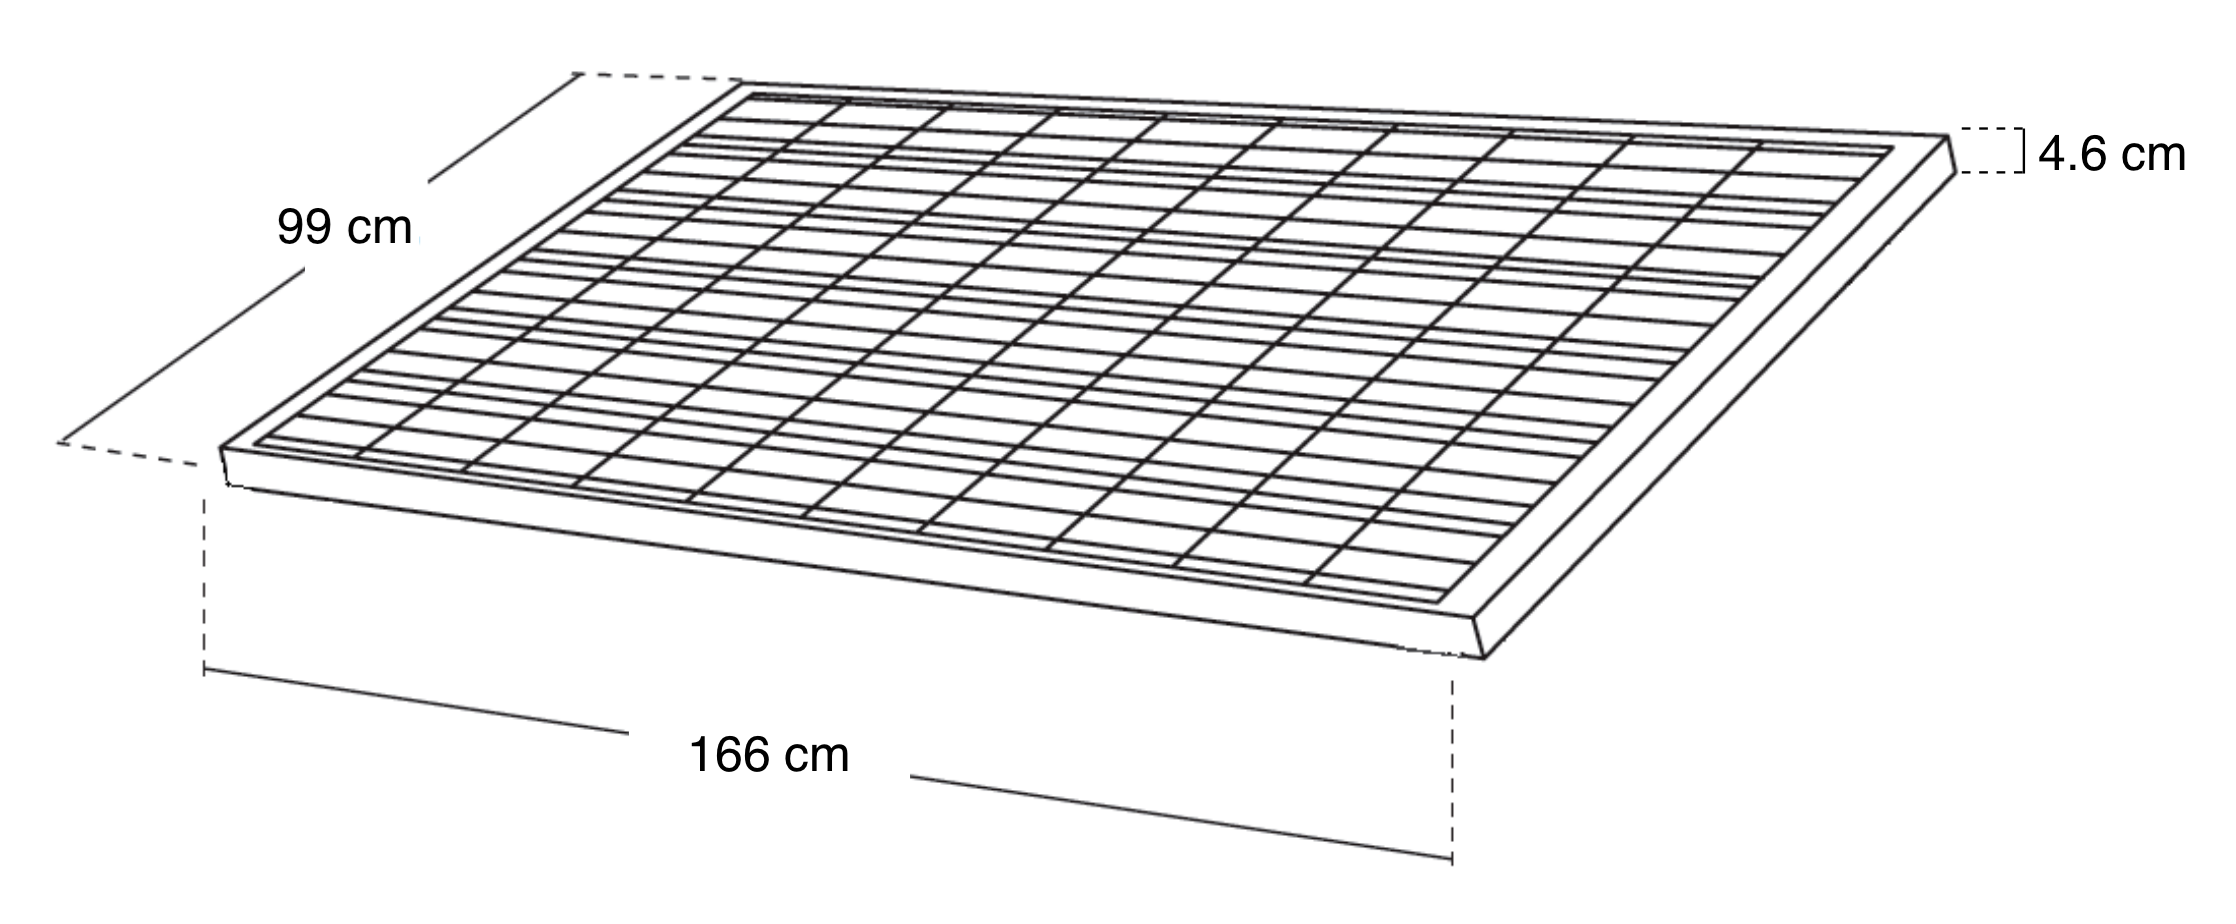
\includegraphics[scale=.25]{Capitulo2/images/panel.png}
	\caption{Módulo Fotovoltaico 250W Policristalino IUSA}
	\label{fig:diagrama_dispensador}
\end{figure}

\paragraph{Microinversor de corriente CC/CA para módulo fotovoltaico M1-01-250}
Diseñado específicamente para interconexiones en el sistema de distribución mexicano, con una salida de 127 V a 60 Hz CA y conector MC4 para conectar el panel solar \citep{MarcoTeorico3}.

\begin{figure}[H]
	\centering
	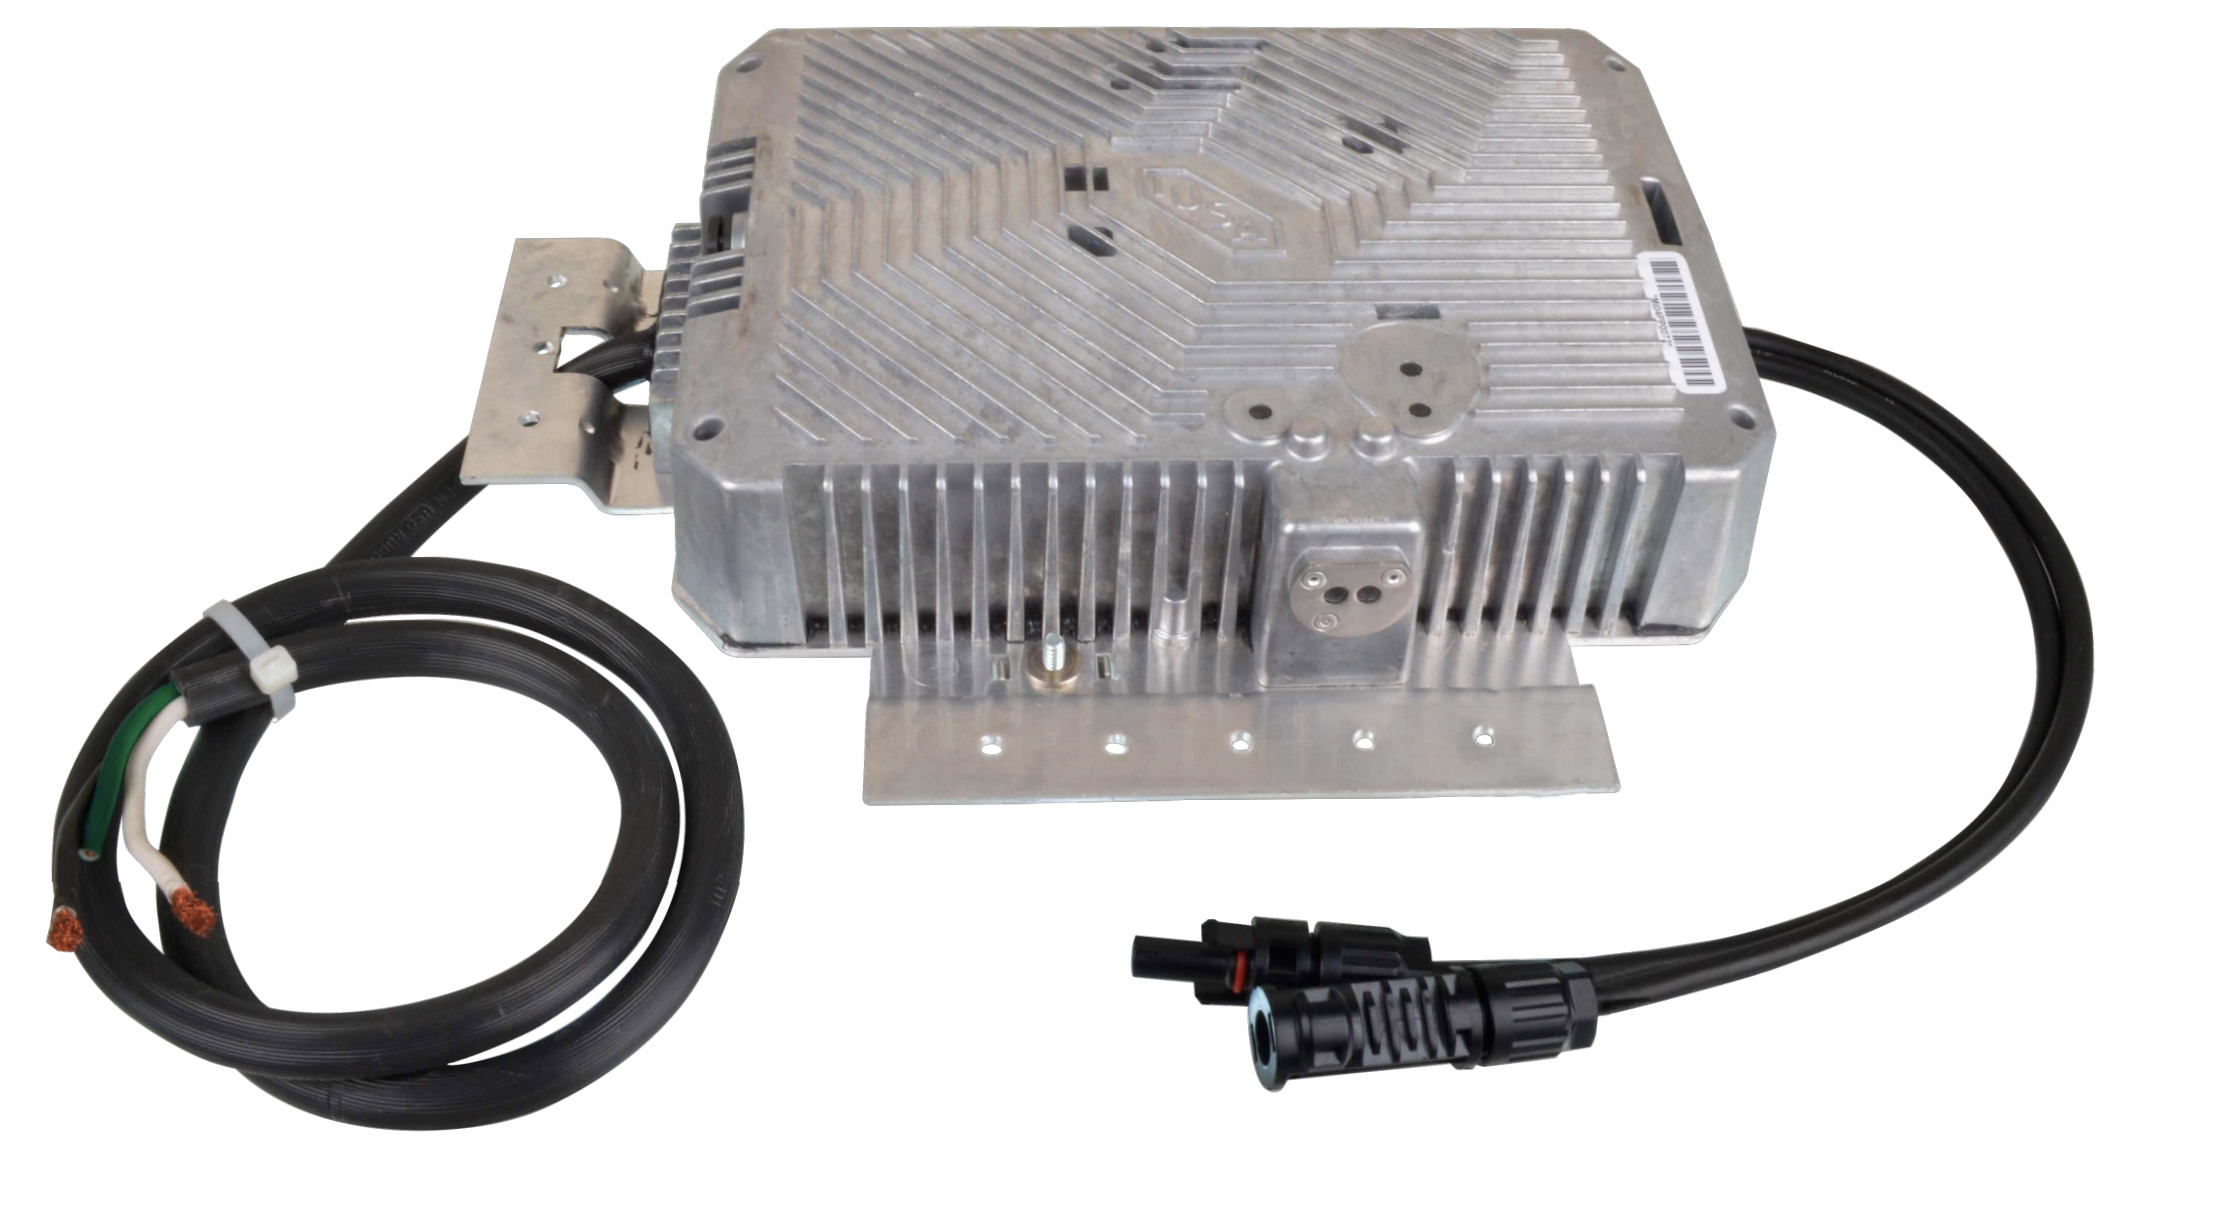
\includegraphics[scale=.20]{Capitulo2/images/microinversor.png}
	\caption{Microinversor M1-01-250}
	\label{fig:diagrama_dispensador}
\end{figure}
 
 
 \section{Wi-Fi}
 \paragraph{}
 Según la Real Academia Española es un sistema de conexión inalámbrica, dentro de un área determinada, entre dispositivos electrónicos, y frecuentemente para acceso a internet. En un sentido literal Wi-Fi no significa nada, es una marca comercial que también es usada para designar a las tecnologías de red sin cable.
 \paragraph{}
 En la actualidad es la que ofrece la mayor cantidad de beneficios al costo más bajo entre todas las tecnologías inalámbricas. Es económica, interoperable con equipos de diferentes fabricantes y puede ser extendida para ofrecer funcionalidades mucho más allá de las previstas originalmente por los fabricantes.
 
 \paragraph{Estándares 802.11}Los estándares inalámbricos son la base de muchos productos inalámbricos, lo que asegura su interoperabilidad y su usabilidad por parte de los que desarrollan, instalan y gestionan redes inalámbricas. Los estándares usados en la mayoría de las redes fueron establecidos por los grupos de trabajo 802 del IEEE. Los equipos de la familia de estándares 802.11 son, con mucho, los más fabricados e instalados para enlaces inalámbricos tanto de interiores como de exteriores. Las interfaces inalámbricas deben concordar en un canal común. Si un dispositivo está sintonizado en el canal 2, mientras que otra lo está en el canal 11, los radios no se podrán comunicar; de esto es lo que se encarga la familia de estándares 802.11 \citep{MarcoTeoricoWifi}.
\paragraph{}
Las redes Wi-Fi poseen una serie de ventajas, entre las cuales podemos destacar:
\begin{itemize}
	\item Al ser redes inalámbricas, la comodidad que ofrecen es muy superior a las redes cableadas porque cualquiera que tenga acceso a la red puede conectarse desde distintos puntos dentro de un espacio lo bastante amplio.
    \item Una vez configuradas, las redes Wi-Fi permiten el acceso de múltiples dispositivos sin ningún problema ni gasto en infraestructura, ni gran cantidad de cables.
    \item Asegura que la compatibilidad entre dispositivos es total, con lo que en cualquier parte del mundo podremos utilizar la tecnología Wi-Fi con una compatibilidad absoluta. 
\end{itemize}
 
 
 
\section{Módulo Wi-Fi MIKROE-2542}

MIKROE-2542 es una placa con un adaptador tipo mikroBUS que integra el módulo ESP-WROOM-02, este último está compuesto por una antena PCB y el chip ESP8266EX \citep{MarcoTeorico5}.

\begin{figure}[H]
	\centering
	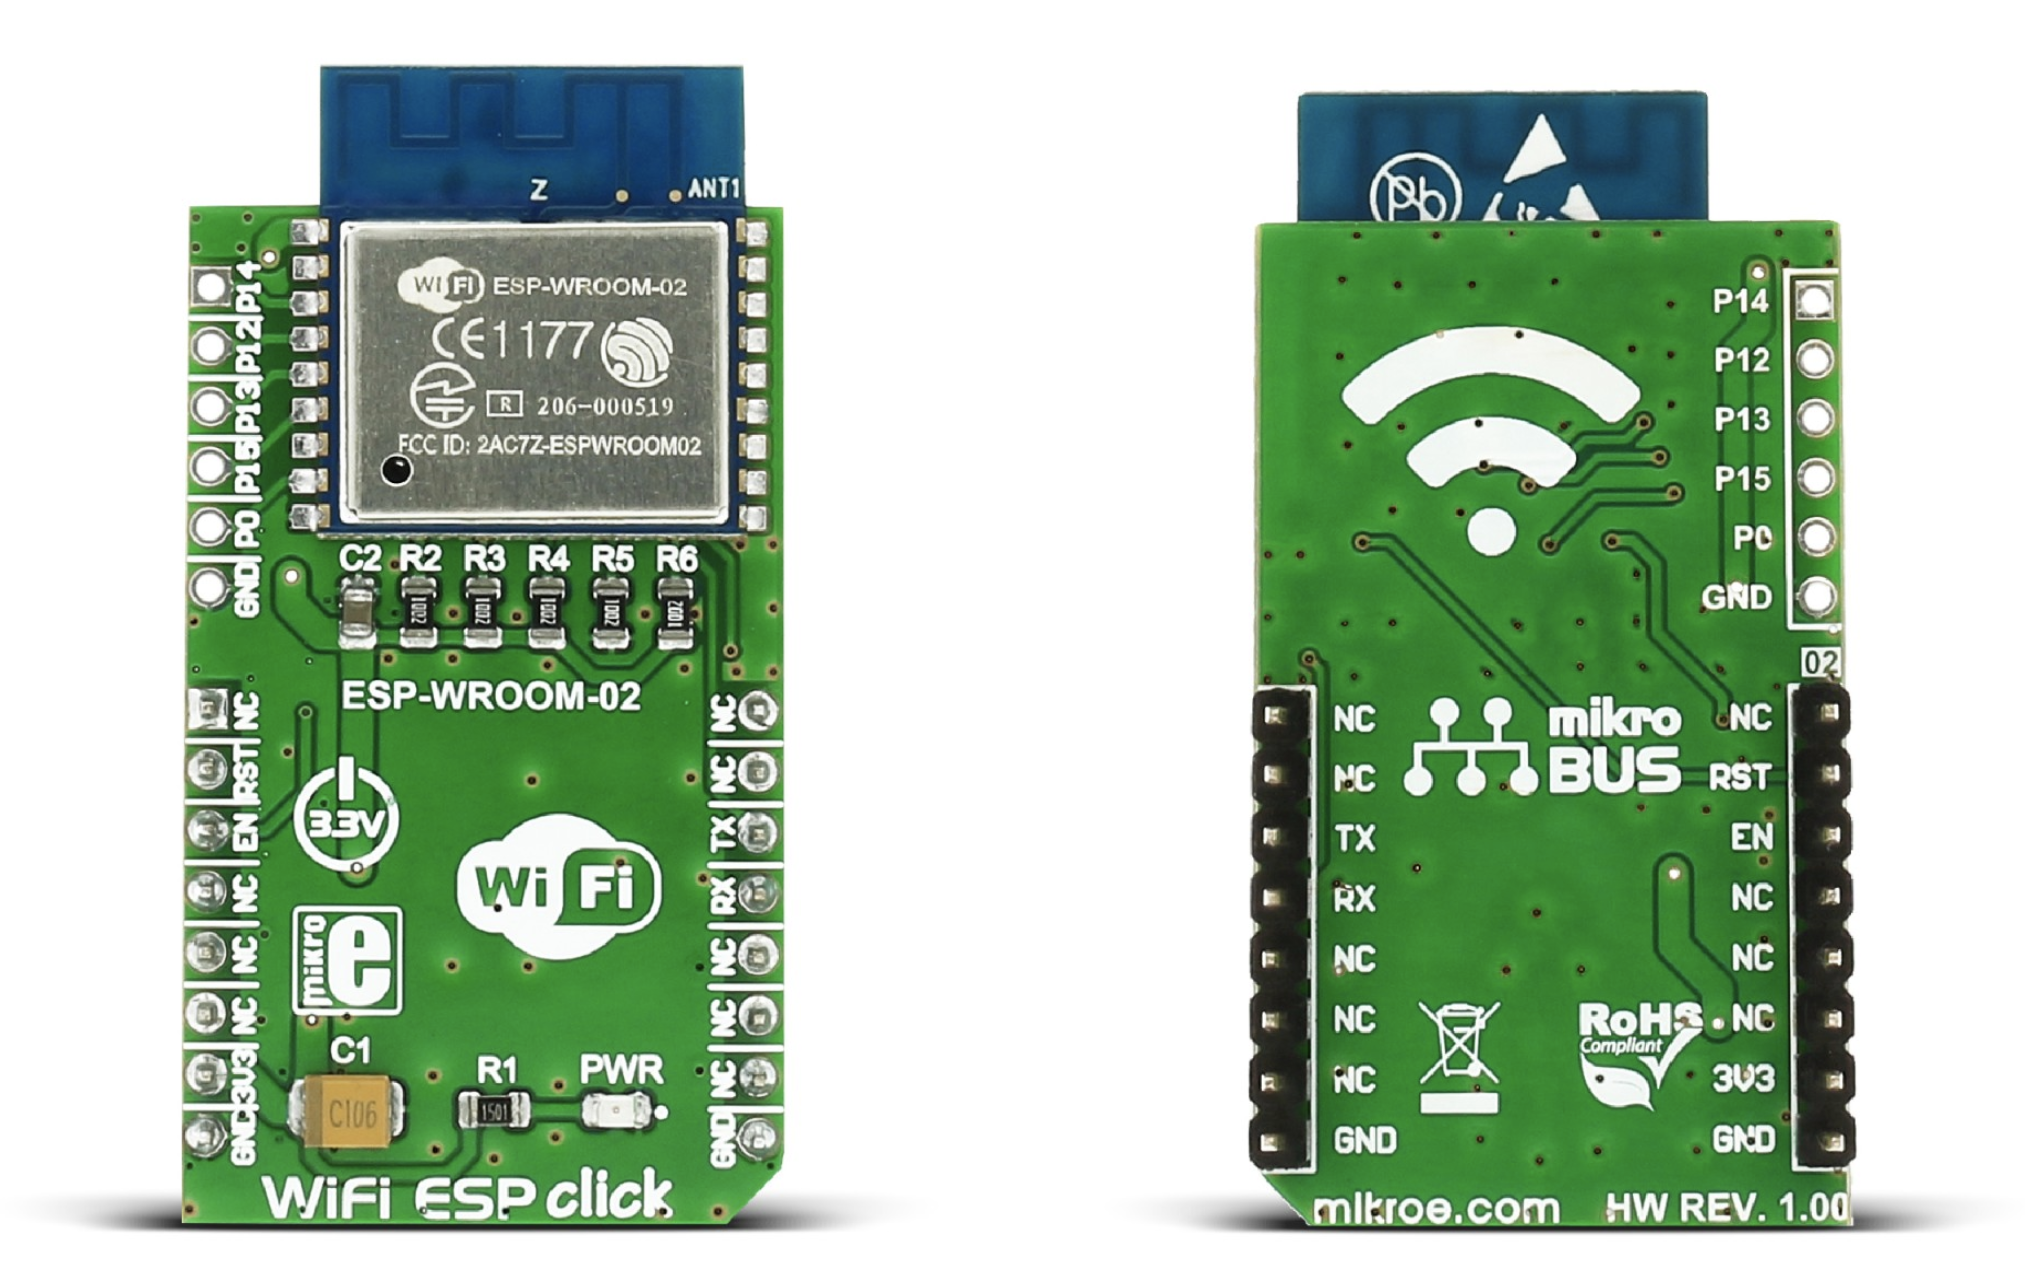
\includegraphics[scale=.4]{Capitulo2/images/mikroe.png}
	\caption{Placa MIKROE-2542, A:frente ; B:posterior}
	\label{fig:diagrama_dispensador}
\end{figure}
\paragraph{}

\begin{figure}[H]
	\centering
	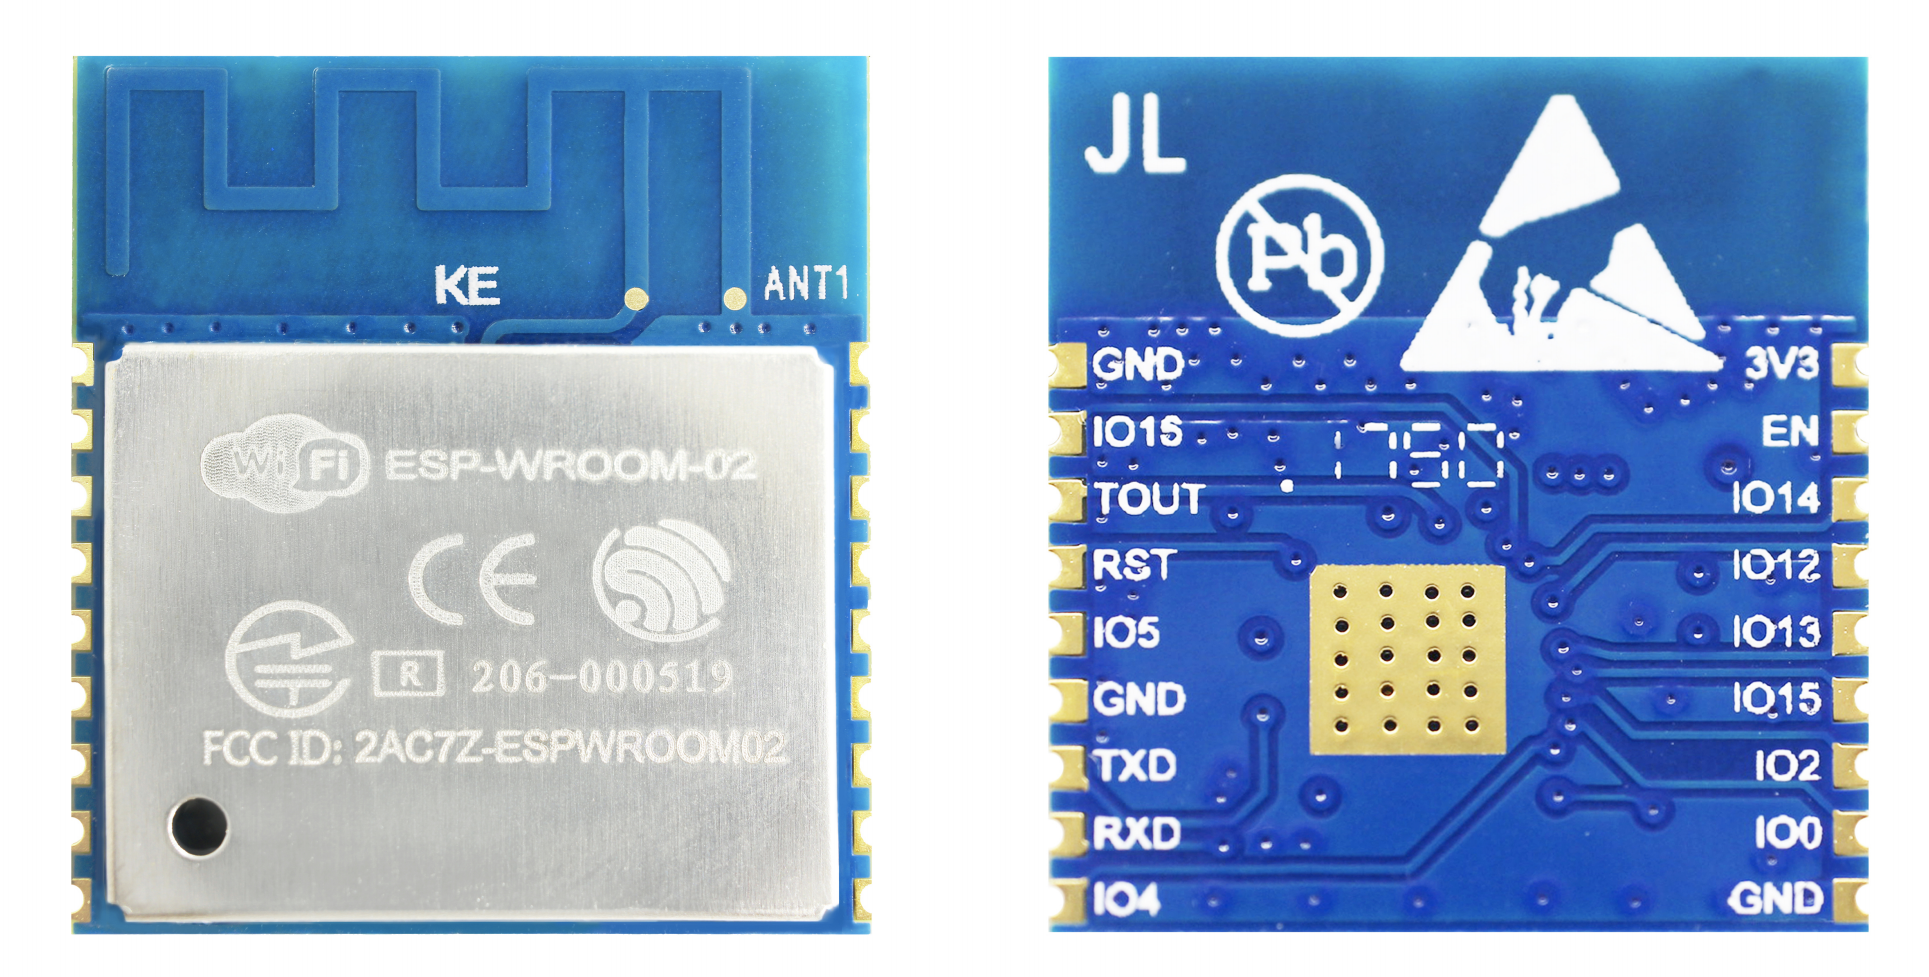
\includegraphics[scale=.2]{Capitulo2/images/wroom.png}
	\caption{Módulo ESP-WROOM-02, A:frente ; B:posterior}
	\label{fig:diagrama_dispensador}
\end{figure}


\paragraph{MikroBUS}
Es un estándar de distribución de los pines para la conexión y comunicación entre un microcontrolador o microprocesador con circuitos integrados o módulos, permitiendo así extender las capacidades de los mismos, este estándar incluye los pines requeridos por las tarjetas de desarrollo más actuales \citep{MarcoTeorico5}.
\begin{figure}[H]
	\centering
	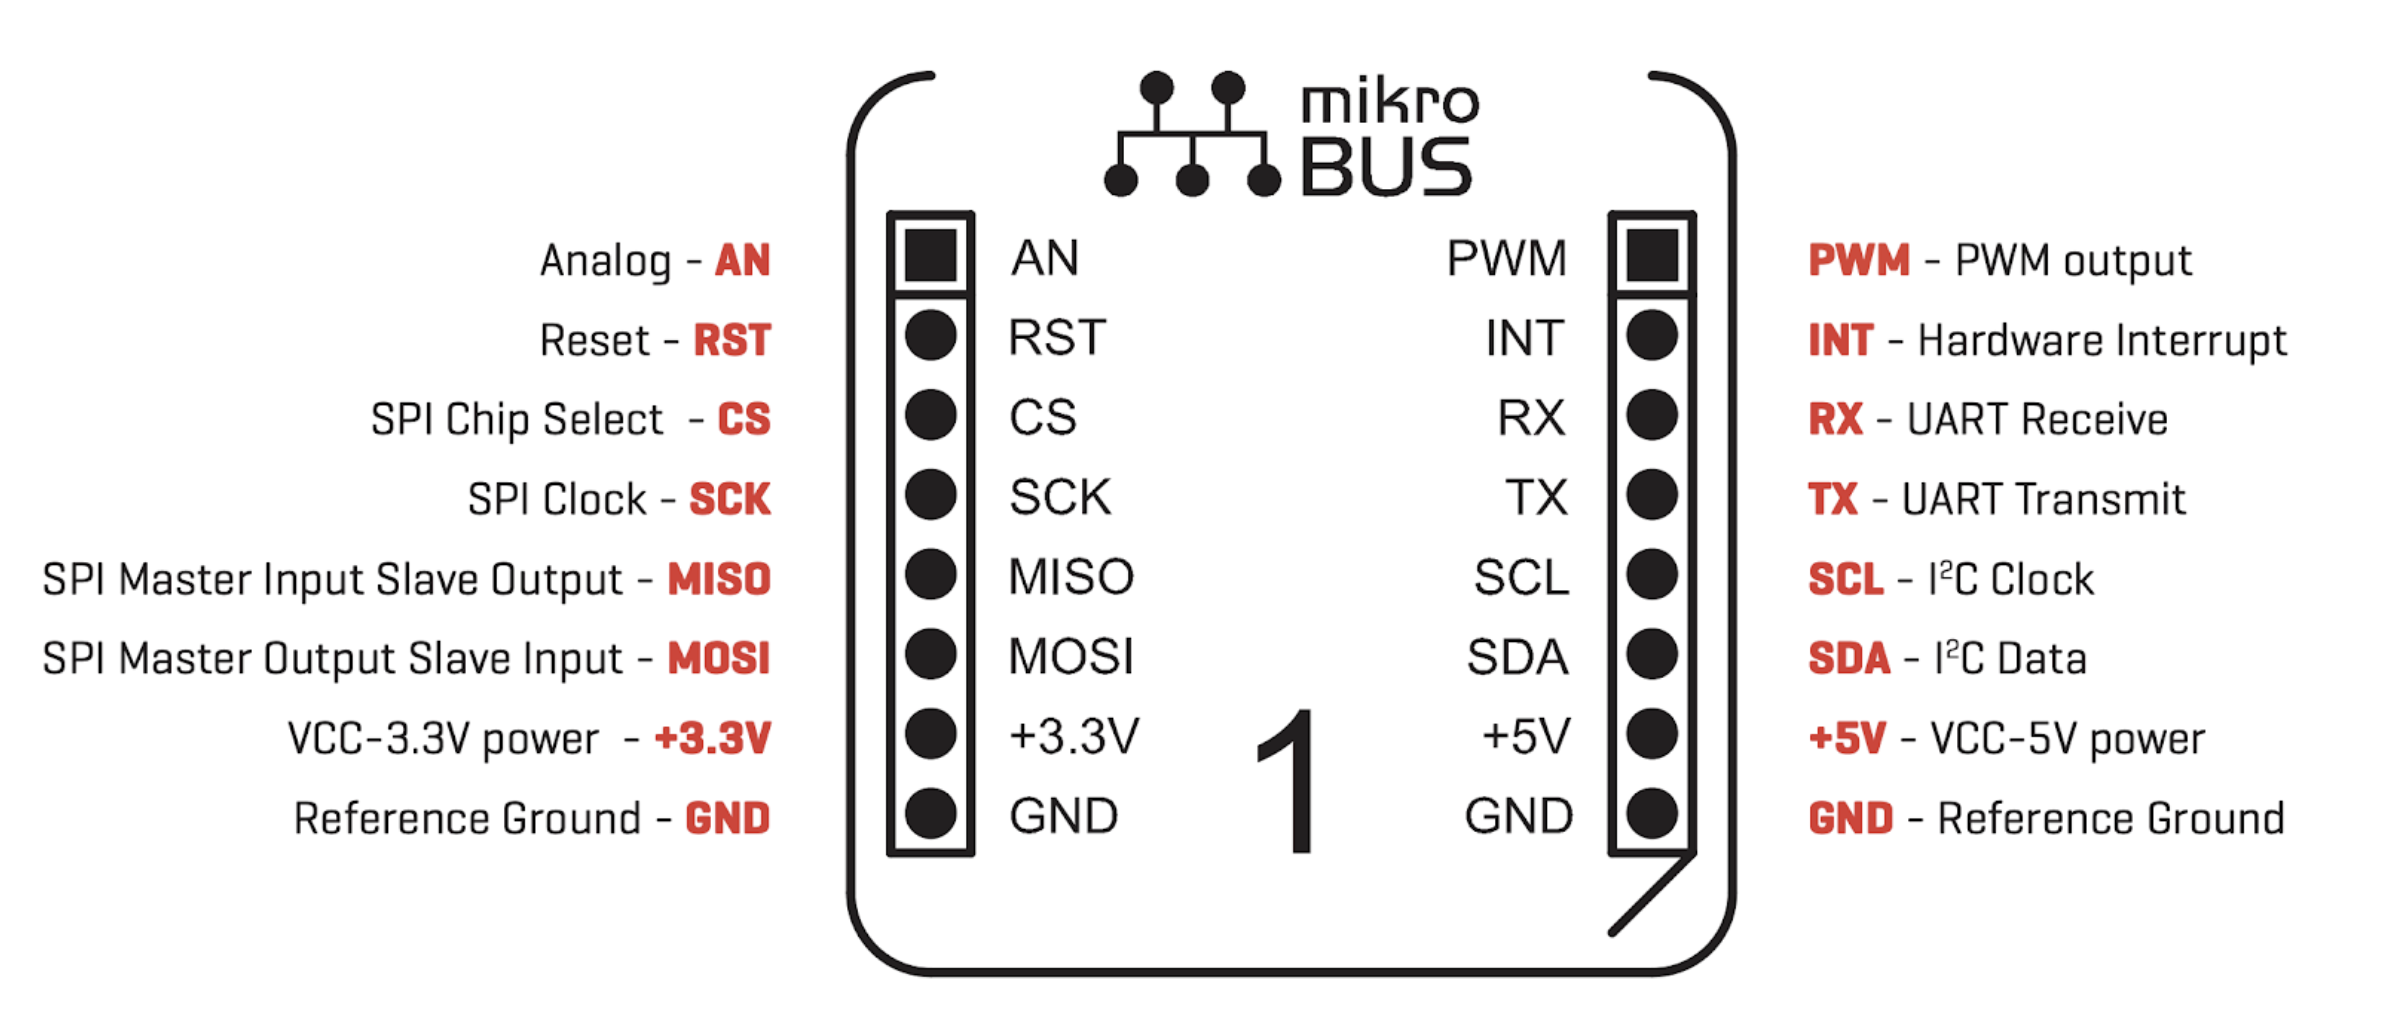
\includegraphics[scale=.25]{Capitulo2/images/mikrobus.png}
	\caption{Distribución de pines tipo MikroBUS}
	\label{fig:diagrama_dispensador}
\end{figure}
\paragraph{}

\paragraph{ESP8266}
El ESP8266 es un SoC Wi-Fi \citep{MarcoTeorico7} (System on Chip: integra todos o gran parte de los módulos que componen un sistema electrónico en un único circuito integrado) compuesto por una pila TCP/IP y un microcontrolador \citep{MarcoTeorico8}.
\paragraph{}

Este módulo permite a otros microcontroladores conectarse a un red inalámbrica Wi-Fi y realizar conexiones simples con TCP/IP haciendo uso eficiente de energía, lo cual lo hace ideal para proyectos de IoT. A continuación, se muestra una comparativa con otros módulos WiFi, la elección de este módulo es debido a que tiene solamente las características de comunicación WiFi necesarias y suficientes para la aplicación a desarrollar.

\begin{figure}[H]
	\centering
	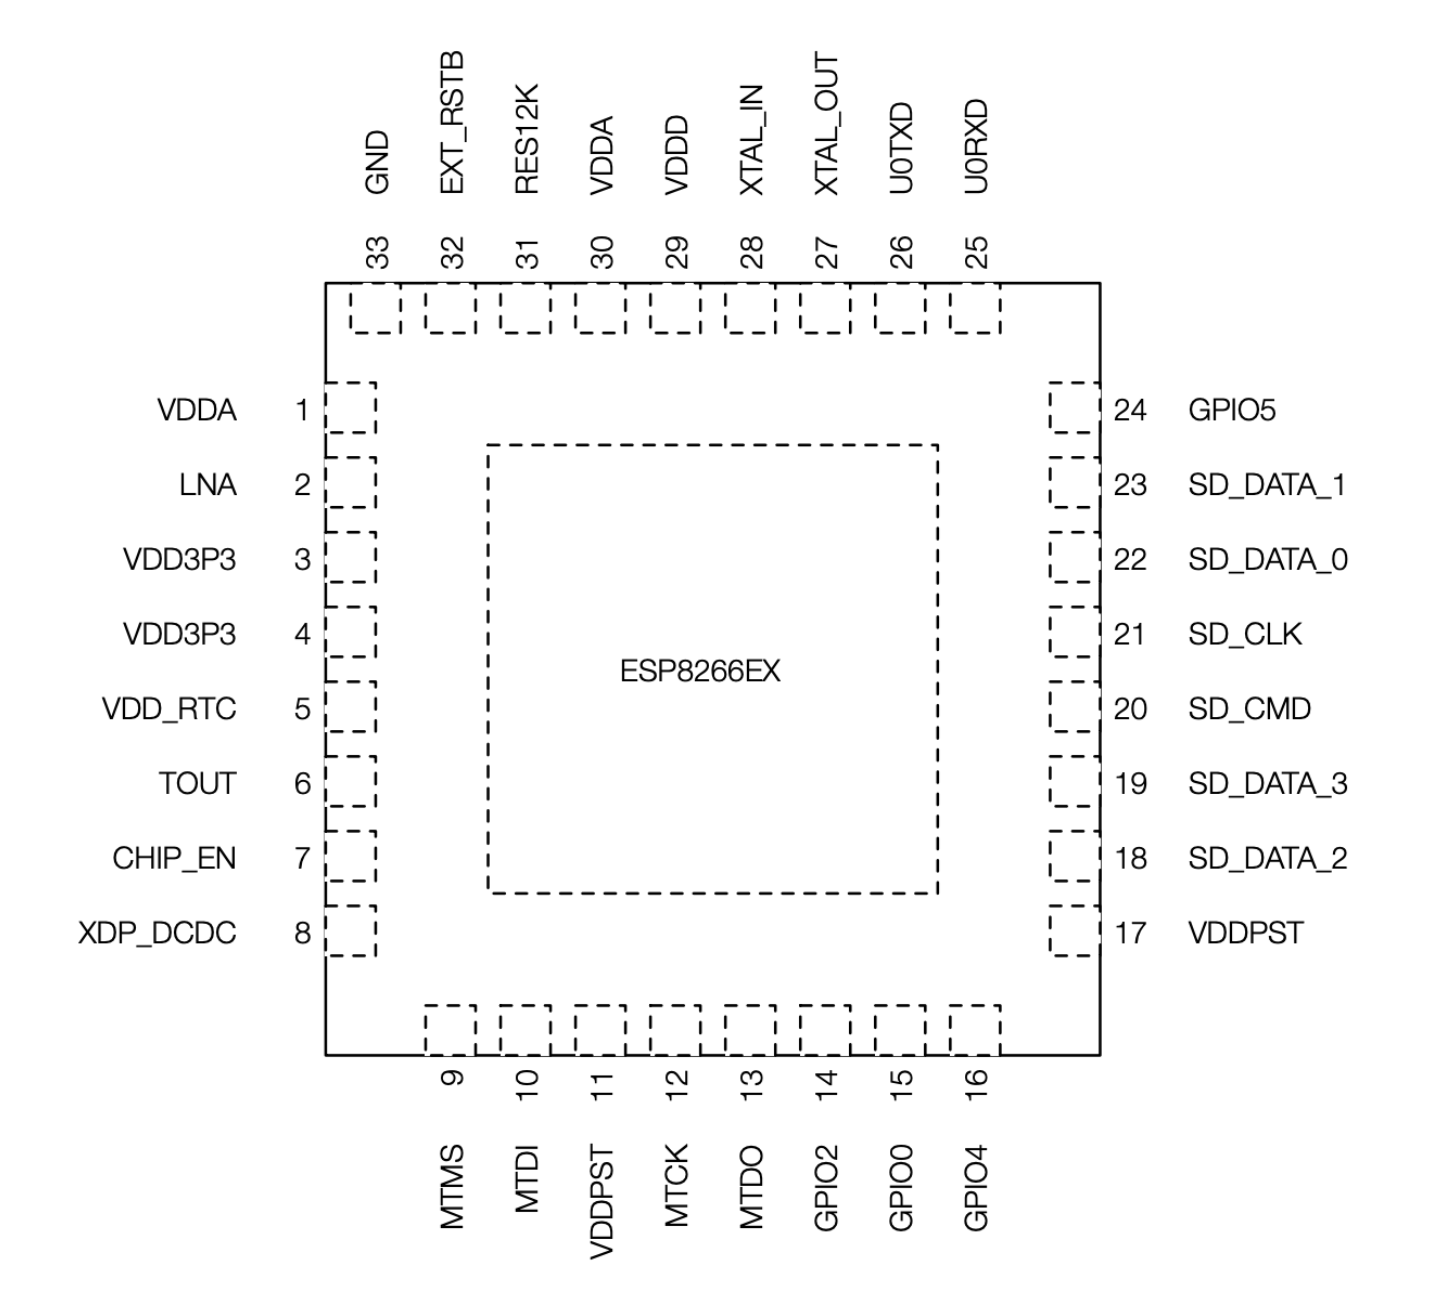
\includegraphics[scale=.3]{Capitulo2/images/esp8266.png}
	\caption{Diagrama esquemático del chip ESP8266}
	\label{fig:diagrama_dispensador}
\end{figure}

\pagebreak

\begin{longtable}{|M{2.2cm}|M{4.0cm}|M{4.0cm}|M{4.0cm}|}
    \caption{Comparativa entre módulos WiFi}
    \label{tabla_modulosWiFi}
	%\centering
	%\begin{tabular}
	\hline
	\textbf{Categoría} & \textbf{MIKROE-2542} & \textbf{356-ESP32-PICO-KIT} & \textbf{GPy 1.0} \\ \hline
	
 	Fabricante & MikroElektronika & Espressif Systems & Pycom
 	\hline
 	 
    Wi-Fi 
    &
    \newline  -Protocolo estándar IEEE 802.11
    \newline  -Rango de frecuencia 2.4G ~ 2.5G 
    \newline  -Antena PCB
	& 
    \newline  -Protoloco estándar IEEE 802.11
    \newline  -Rango de frecuencia 2.4G ~ 2.5G 
    \newline  -Antena 3D
	&   	    
    \newline  -Protoloco estándar IEEE 802.11
    \newline  -Rango de frecuencia 2.4G ~ 2.5G 
    \newline  -Antena Bluetooth y WiFi interna
    \newline  -Conector para antena LTE CAT M1 / NB1
    \newline  -Transceiver LTE CAT M1/ NB1 	
    \hline

	Bluetooth 
    &
	---
    &
	\newline Protocolo Bluetooth V4.2
	&
	\newline Protocolo Bluetooth V4.2 
	\hline
	
	Hardware &
    \newline  -CPU Tensilica L106 32-bit processor
    \newline  -Interfaz Periférica UART/SDIO/SPI/IIC/I2S/IR Control Remoto
    \newline  -Intefaces GPIO/ADC/PWM/LED Light
    \newline  -Voltaje de operación entre 2.5V ~ 3.6V
    &
    \newline  -CPU ESP32-PICO-D4
    \newline  -Interfaz Periférica ADC, DAC, sensor touch, SD/SDIO/MMC Host Controller, SPI, SDIO/SPI Controlador Esclavo, EMAC, motor PWM, LED PWM, UART, IIC, I2S, Control Remoto Infrarojo 
    \newline  -Voltaje de operación entre 2.5V ~ 3.6V
    \newline  -Sensor Hall integrado
    \newline  -Cristal de 40 MHz
    \newline  -SPI flash de 4MB integrada
    &
    \newline  - CPU Espressif ESP32 SoC
    \newline  - Coprocesador ULP
    \newline  - Interfaz Periférica ADC Controller
    \newline  - Voltaje de operación entre 2.5V ~ 3.6V
    \newline  - Memoria flash de 8MB integrada
    &
	\hline
	
    Precio (USD) & \$ 19.50 & \$ 13.00 & \$ 71.40
    \hline
	
	% \end{tabular}
	%\label{tabla_riesgos}
\end{longtable}

\pagebreak

\paragraph{}

\section{IoT (Internet de las cosas)}
De acuerdo con la definición otorgada por la IEEE, el internet de las cosas o IoT, es un dominio de aplicación que integra diferentes tecnologías y campos sociales, a pesar de la diversidad de las investigaciones sobre IoT \citep{MarcoTeoricoIoT}. El Internet de las cosas (IoT) se está convirtiendo en un tema de conversación cada vez más creciente tanto en el lugar de trabajo como fuera de él. Es un concepto que no sólo tiene el potencial de impactar cómo vivimos, sino también cómo trabajamos. 
\paragraph{}
El Internet de banda ancha está cada vez más disponible, el costo de la conexión reduciendo, se están creando más dispositivos con capacidades Wi-Fi y sensores integrados, los costos de la tecnología están disminuyendo y la penetración de los teléfonos inteligentes disparando. En pocas palabras, este es el concepto de conectar básicamente cualquier dispositivo con un interruptor de encendido y apagado a Internet. Esto incluye todo, desde teléfonos celulares, cafeteras, lavadoras, audífonos, lámparas, dispositivos portátiles y casi cualquier otra cosa que se pueda imaginar. Esto también se aplica a los componentes de las máquinas. La firma de analistas Gartner dice que para 2020 habrá más de 26 mil millones de dispositivos conectados. El IoT es una red gigante de cosas conectadas (que también incluye a las personas). La relación será entre personas-personas, personas-cosas y cosas-cosas.
\paragraph{}
Hay muchos ejemplos de cómo podría verse esto o cuál podría ser el valor potencial. Digamos, por ejemplo si se está en camino a una reunión; el automóvil podría tener acceso a su calendario y ya sabe cuál es la mejor ruta a seguir. Si el tráfico es intenso, el automóvil podría enviar un mensaje de texto a la otra parte notificándole que llegará tarde. 
\paragraph{}
La realidad es que el IoT permite oportunidades y conexiones virtualmente infinitas, muchas de las cuales ni siquiera podemos pensar o entender completamente su impacto. Ciertamente abre la puerta a muchas oportunidades pero también a muchos desafíos. La seguridad es un gran problema que a menudo se plantea. Luego tenemos el tema de la privacidad y el intercambio de datos. Este es un tema candente incluso hoy en día, por lo que sólo se puede imaginar cómo la conversación y las preocupaciones aumentarán cuando se habla de la conexión de muchos miles de millones de dispositivos \citep{MarcoTeoricoIoT2}. 



\section{Demonio / Servicio}
Un demonio o servicio es un programa que se ejecuta en segundo plano, fuera del control interactivo de los usuarios del sistema, ya que carecen de interfaz con estos. El término demonio se usa fundamentalmente en sistemas UNIX y basados en UNIX, como GNU/Linux o Mac OS X \citep{MarcoTeorico4}.

\section{Yocto}
Yocto Project (YP) es un proyecto de colaboración de código abierto que ayuda a los desarrolladores a crear sistemas personalizados basados en Linux, independientemente de la arquitectura del hardware.
\paragraph{}
El proyecto proporciona un conjunto flexible de herramientas y un espacio donde desarrolladores de todo el mundo pueden compartir tecnologías, pilas de software, configuraciones y mejores prácticas que se pueden usar para crear imágenes de Linux personalizadas para dispositivos IoT e integrados, o en cualquier lugar donde se necesite un sistema operativo Linux personalizado \citep{MarcoTeoricoYocto}.
\paragraph{}
De igual manera proporciona un estándar para entregar soporte de hardware y pilas de software, permitiendo el intercambio de configuraciones y compilaciones de software. Las herramientas permiten a los usuarios crear y admitir personalizaciones para múltiples plataformas de hardware y pilas de software de una manera mantenible y escalable.
\paragraph{}
Un conjunto de herramientas integradas para que el trabajo con Linux incorporado sea exitoso, que incluye herramientas para la creación y prueba automatizadas, procesos para el soporte de la placa y el cumplimiento de licencias e información de componentes para sistemas operativos integrados basados en Linux personalizados.
\paragraph{OpenEmbedded}
El sistema de compilación OpenEmbedded, mantenido conjuntamente con el proyecto OpenEmbedded, que es donde se derivan el sistema de compilación y algunos de los metadatos, los cuales se usan para construir una distribución de Linux, contenida en los archivos que el sistema de compilación analiza al crear una imagen. En general, los metadatos incluyen archivos de configuración y otra información relacionada con las propias instrucciones de compilación, así como los datos utilizados para controlar qué cosas se construyen y cómo se construyen. Los metadatos también incluyen comandos y datos utilizados para indicar qué versiones de software se utilizan y de dónde se obtienen, así como cambios o adiciones al software en sí (parches o archivos auxiliares) que se utilizan para corregir errores o personalizarlos.
\paragraph{}
A continuación, mencionamos algunas de las características de Yocto Project:
\begin{itemize}
	\item El proyecto Yocto se adopta ampliamente en toda la industria integrada / IoT.
    \item Yocto Project funciona en cualquier arquitectura.
    \item No está limitado a ningún proveedor ya que Yocto Project es tanto de código abierto como compatible con muchas arquitecturas.
    \item La salida de Yocto Project es fácilmente transferible a otra arquitectura, lo que le permite tener líneas de productos que utilizan diversas arquitecturas sin obligarlo a intercambiar entornos de desarrollo.
    \item El Proyecto Yocto se valida constantemente al probar todas las versiones con la distribución de referencia (Poky) en cada arquitectura compatible.
\end{itemize}
\paragraph{}
Yocto Project tiene un modelo de desarrollo IoT de Linux que lo distingue de otros sistemas de compilación simple. Se llama el modelo de capa.
\paragraph{}
El modelo de capa está diseñado para admitir la colaboración y la personalización al mismo tiempo. Las capas son repositorios que contienen conjuntos de instrucciones relacionados que le indican al sistema de compilación qué hacer. Los usuarios pueden colaborar, compartir y reutilizar capas. Las capas pueden contener cambios a las instrucciones o configuraciones anteriores en cualquier momento \citep{MarcoTeoricoYocto2}.


\section{Dispositivo de monitoreo de energía}
En este trabajo se plantea el uso de un dispositivo de monitoreo de energía que permita supervisar de manera constante la energía producida por un sistema fotovoltaico; es por ello que a continuación definiremos algunos conceptos importantes.
\paragraph{}
Inicialmente, un dispositivo puede ser definido como un mecanismo dispuesto para obtener un resultado automático \citep{MarcoTeorico11}; es decir, un conjunto de elementos bien definidos, que entre sí, realizan acciones conforme la información recibida (entrada) para poder transformarla (salida).
Existe una amplia gama de clasificación de dispositivos de acuerdo al propósito para el que es empleado, sin embargo, para fines de este trabajo, el dispositivo de interés entra en la categoría de aquellos que se encargan de monitorear. 
\paragraph{}
De acuerdo a la Real Academia Española, la palabra monitorear, se define como la acción de observar, supervisar o controlar mediante aparatos especiales, el curso de uno o varios parámetros fisiológicos o de otra naturaleza para detectar posibles anomalías \citep{MarcoTeorico12}.
\paragraph{}
Teniendo en cuenta los 2 conceptos anteriores, podemos definir a un dispositivo de monitoreo de energía como: un mecanismo que recibe como entrada energía e internamente procesa dicha información para finalmente arrojar datos de monitoreo.
\paragraph{MCP39F521}
El dispositivo que se usará es el MCP39F521 (I2C Power Monitor with Calculation and Energy Accumulation), el cual se define como un dispositivo de alta integración de monitoreo de energía de fase completa, diseñado para realizar medición en tiempo real de la energía de entrada para las fuentes de alimentación de corriente directa o alterna, unidades de distribución de energía y aplicaciones de consumidor e industriales. Una de las características de este dispositivo que importa señalar, es que cuenta con una interfaz IIC, como se puede observar en el siguiente diagrama, dicha interfaz tiene una velocidad de reloj de hasta 400 kHz \citep{MarcoTeorico13}; de esta forma es como se realizará la comunicación que permita el intercambio de la información monitoreada con el microcontrolador. 
\paragraph{}
\begin{figure}[H]
	\centering
	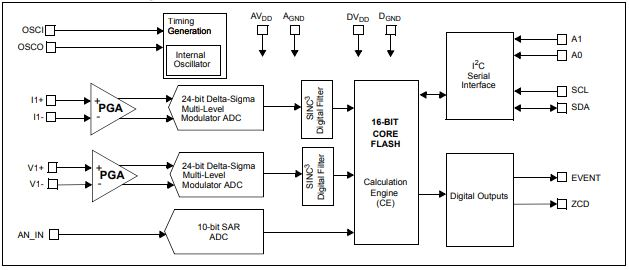
\includegraphics[scale=.9]{Capitulo2/images/DiagramaDispMonitoreo.JPG}
	\caption{Diagrama a bloques del MCP39F521}
	\label{fig:diagrama_dispMonitoreo}
\end{figure}

\paragraph{IIC}
IIC es una interfaz serial síncrona de comunicación, la cual es útil para comunicarse  con otros periféricos y microcontroladores, fue desarrollada por Philips Semiconductors.
Estos periféricos pueden ser: Memorias seriales EEPROMS, registros de corrimiento, expansores de puerto, ADC's, DAC's, entre otros \citep{MarcoTeorico17}.
\paragraph{}
Sólo se utilizan dos líneas para comunicación:
\begin{itemize}
	\item Una línea de datos serial (SDA)
    \item Una línea de reloj serial (SCL), que siempre es generada por el maestro.
\end{itemize}

Cada dispositivo conectado al bus es reconocido por una única dirección, el bus maneja una arquitectura maestro-esclavo, el maestro trabaja como transmisor o receptor, donde el maestro inicia y termina la transferencia de información.

\begin{figure}[H]
	\centering
	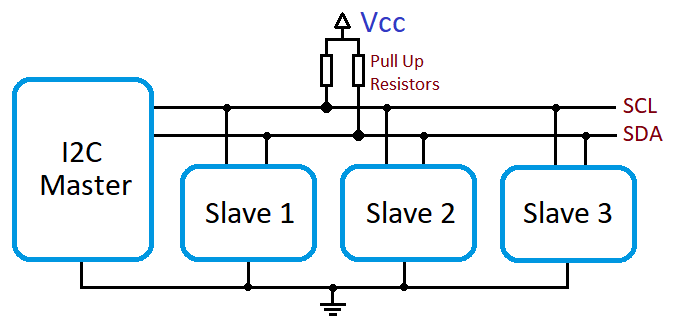
\includegraphics[scale=.35]{Capitulo2/images/I2C-Interface.png}
	\caption{Diagrama ejemplificativo de interfaz IIC}
	\label{fig:}
\end{figure}

Entre las características principales están:
\begin{itemize}
	\item Se realizan transferencias seriales bidireccionales de 8 bits.
    \item Se proporciona filtrado en Chip para eliminar picos en la línea de datos y preservar integridad de datos.
    \item El número de circuitos integrados que pueden ser conectados al bus está limitado a la capacitancia máxima del bus.
    \item Modo estándar de operación (Standard Mode). Con velocidad de hasta 100 kbps.
    \item Modo rápido de operación  (Fast mode). Con velocidad de hasta 400 kbps. \item Modo más rápido de operación (Fast mode plus). Con velocidad de hasta 1 Mbps.
\end{itemize}

Para que la transferencia de información pueda ser iniciada, el bus debe estar libre. Todas las transacciones comienzan con START y pueden ser terminadas por un STOP.
Una transición de alto a bajo en la línea SDA mientras SCL es alto, define una condición de START.
Una transición de bajo a alto en la línea SDA mientras SCL es alto, define una condición de STOP.

\begin{figure}[H]
	\centering
	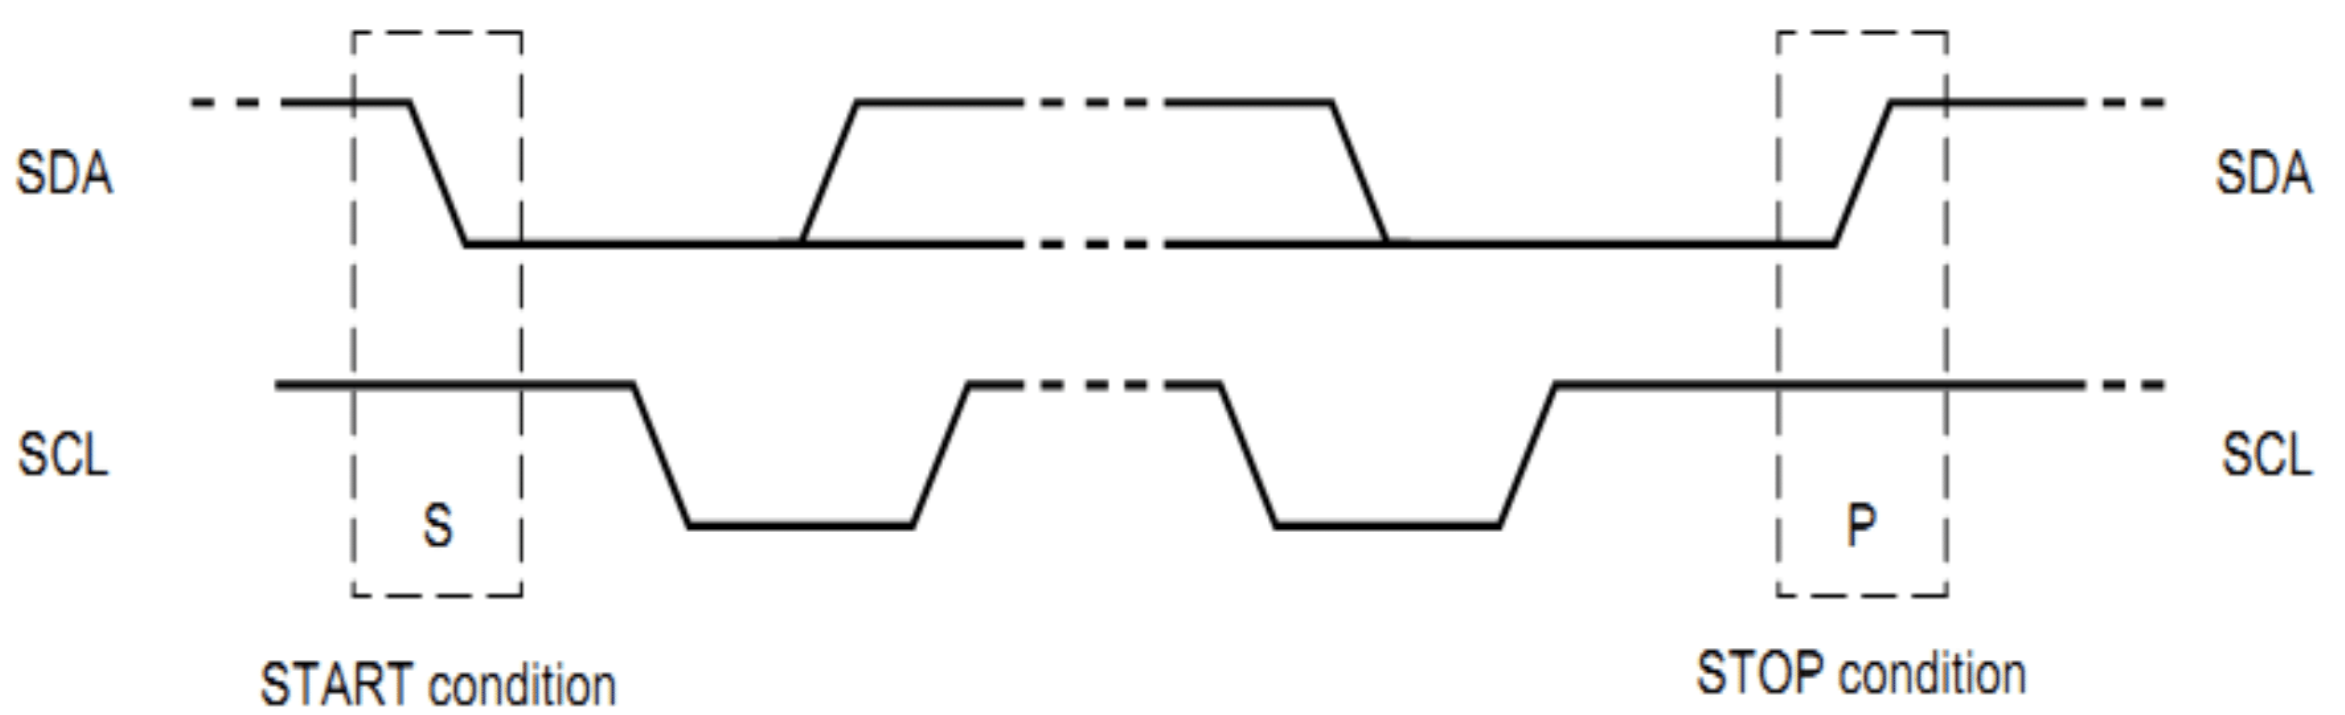
\includegraphics[scale=.25]{Capitulo2/images/startstop.png}
	\caption{Protocolo de START y STOP}
	\label{fig:}
\end{figure}



\section{Sistema Embebido}
Un sistema embebido es un dispositivo diseñado para un propósito en específico, el cual abarca desde una operación hasta un conjunto pequeño de operaciones en tiempo real, a diferencia de una PC, la cual puede realizar una gran cantidad de tareas de acuerdo a los programas que se ejecuten. 
\paragraph{}
El uso de los sistemas embebidos ha cobrado gran importancia debido a los usos y aplicaciones que se le han dado, como son: hornos de microondas, máquinas expendedoras, routers, cámaras digitales, reproductores MP3, entre otros. 
\paragraph{}
Algunas de las características principales de los sistemas embebidos son: que tienden a ser de dimensiones pequeñas, son considerados económicos o de bajo costo, su nivel de consumo eléctrico es bajo, poseen recursos limitados de memoria así como de dispositivos de entrada/salida \citep{MarcoTeorico14}.
\paragraph{}
Por lo general, los sistemas embebidos al ofrecer como ventaja la realización de operaciones en tiempo real, suelen ser empleados en ambientes físicos donde se hace uso de sensores y actuadores. Se dice que son sistemas reactivos, pues están en interacción continua con su entorno y el ritmo de su ejecución está coordinada con dicho entorno. 
\paragraph{}
Los sistemas embebidos suelen tener en una de sus partes una computadora con características especiales conocida como microcontrolador que viene a ser el cerebro del sistema, el cual incluye interfaces de entrada/salida en el mismo chip. Normalmente estos sistemas poseen una interfaz externa para efectuar un monitoreo del estado y hacer un diagnóstico del sistema \citep{MarcoTeorico15}.
\paragraph{}
Los sistemas embebidos pueden ser implementados en placas únicas (SBC) y sobre estas se encuentran integrados los recursos de hardware como el microprocesador, la memoria RAM, controladores Ethernet, etc \citep{MarcoTeorico14}.
\paragraph{SBC}
SBC por sus siglas en inglés, Single Board Computer es, como su nombre lo indica, una Computadora de Placa Única, lo cual implica que tiene la totalidad o cumple con la mayoría de las características que tienen las computadoras personales pero en una placa de circuito; sin embargo al tratarse de una placa, es de menores dimensiones así como de un precio relativamente más bajo.
\paragraph{}
Dependiendo el tipo de SBC, pueden llegar a ejecutar como Sistema Operativo Linux, Android o Windows. También cuentan con puertos de Entrada/Salida de propósito general, los cuales permiten la comunicación con otros dispositivos \citep{MarcoTeorico18}. 
\paragraph{}
Algunos ejemplos de SBC son la Raspberry Pi, Banana Pi, BeagleBone Black, PcDuino, entre otros.
\paragraph{Raspberry Pi}
En este trabajo, haremos uso de la Raspberry Pi. Como se menciona en el párrafo anterior, es una SBC. Fue desarrollada en el Reino Unido por la fundación Raspberry Pi con el propósito de promover la educación informática en las escuelas. Algunas de sus principales características son: corre en el sistema operativo Linux así como en Raspbian y Pidora, las cuales son distribuciones de Linux; además tiene conexión a monitor, teclado y mouse \citep{MarcoTeorico19}.   

A continuación, se muestra una comparativa entre la Raspberry Pi 3B y la Banana Pi M2 Berry \citep{MarcoTeorico21}\citep{MarcoTeorico22}.

\begin{figure}[H]
	\centering
	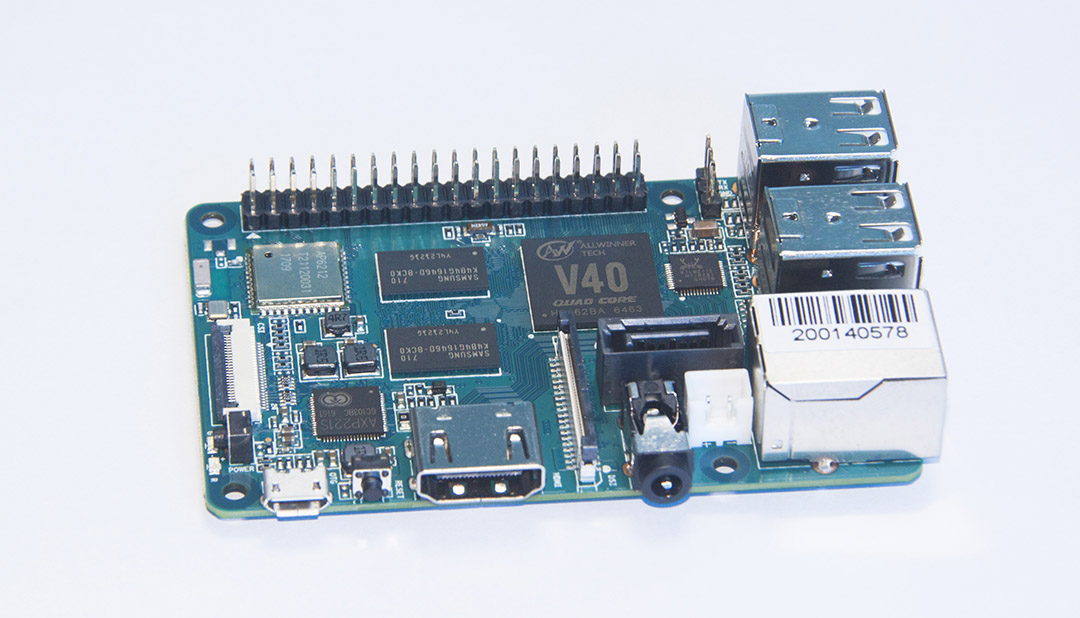
\includegraphics[scale=.8]{Capitulo2/images/bananaPi.jpg}
	\caption{Banana Pi M2 Berry}
	\label{fig:diagrama_dispMonitoreo}
\end{figure}

\paragraph{}
\begin{figure}[H]
	\centering
	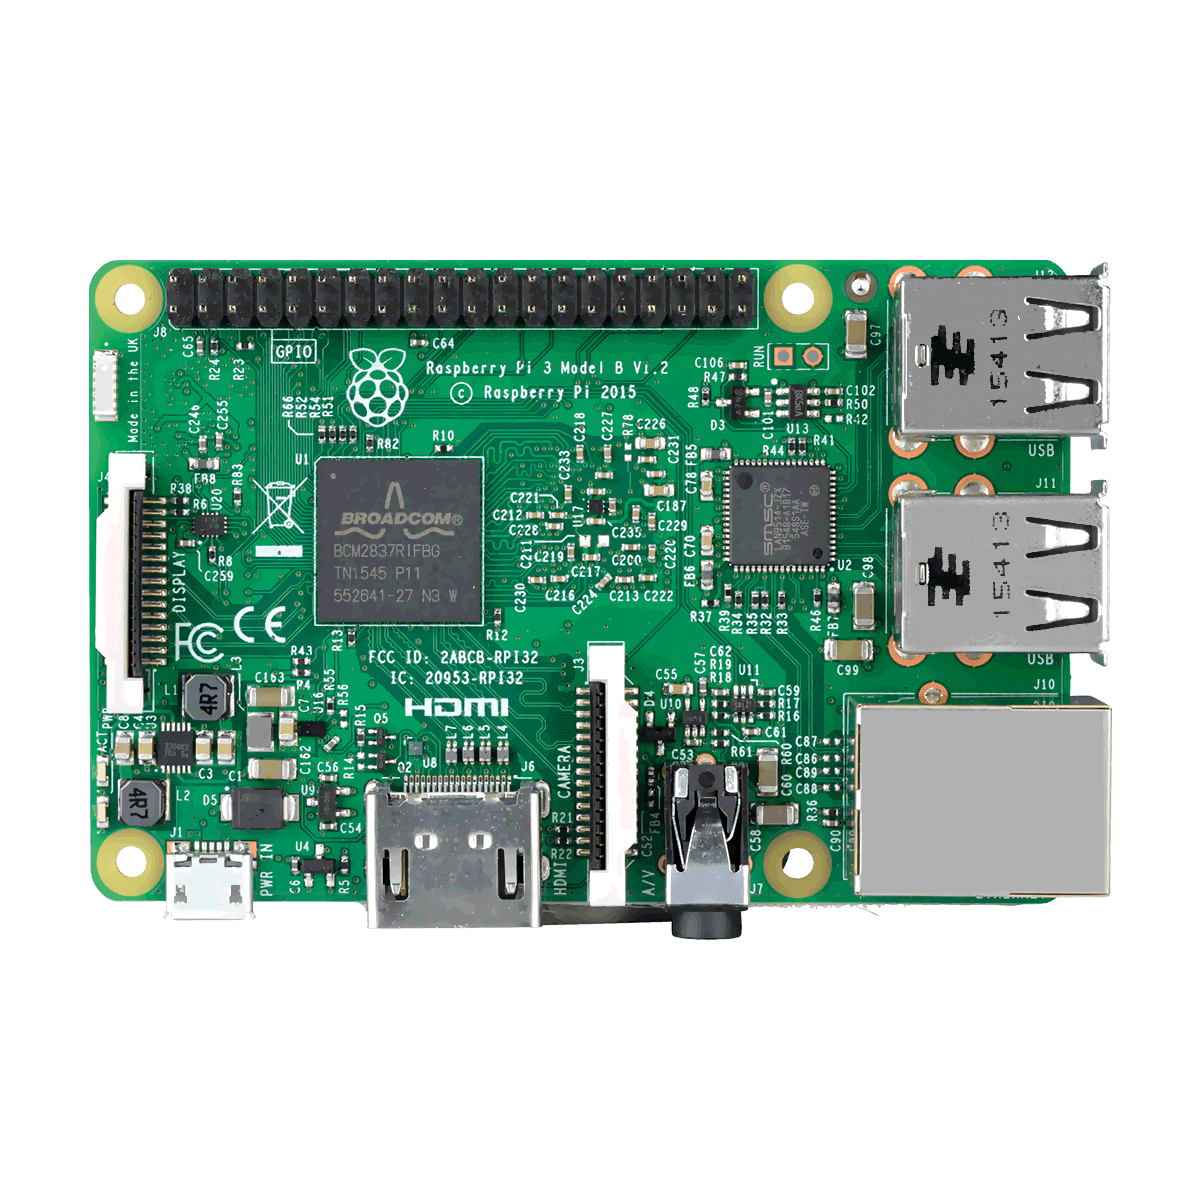
\includegraphics[scale=.23]{Capitulo2/images/raspberry.png}
	\caption{Raspberry Pi 3B}
	\label{fig:diagrama_dispMonitoreo}
\end{figure}

\pagebreak
\begin{longtable}{|M{3.0cm}|M{4.5cm}|M{4.5cm}|}
    \caption{Comparativa entre Banana Pi M2 Berry y Raspberry Pi 3B}
%\begin{table}[!hbt]
	% \centering
	 %\begin{tabular}{|M{3.0cm}|M{4.5cm}|M{4.5cm}|}
	\hline
	\textbf{Característica} & \textbf{Banana Pi M2 Berry} & \textbf{Raspberry Pi 3B} \\ 
	\hline
 	Procesador & Quad Core ARM Cortex A7 V40 & Quad Core 64bit ARM Cortex A53 1.2GHz \\
 	\hline
    GPU & 500 MHz Mali-400 MP2 & 400 MHz VideoCore IV multimedia\\
    \hline
    RAM & 1GB DDR3 SDRAM & 1GB LPDDR2-900 SDRAM \\
	\hline
	Tarjeta de Red & 10/100/1000 Mbps Ethernet y 802.11 b/g/n & 10/100 Mbps Ethernet y 802.11n Wireless LAN\\
	\hline
	Almacenamiento & Micro SD (hasta 64 GB) & Micro SD\\
	\hline
	Salida Video & HDMI, MIPI DSI para paneles LCD & HDMI\\
    \hline
    Salida Audio 
    & 
    \newline - HDMI 
    \newline - Jack 3.5 mm 
    & 
    \newline - HDMI
    \newline - Jack 3.5 estéreo \\
    \hline
    USB & 
    \newline - 4x USB 2.0 
    \newline - USB OTG(Micro USB) 
    & 
    \newline - 4x USB 2.0
    \newline - 1x micro USB alimentación \\
    \hline
    Sistema Operativo 
    & 
    \newline - Raspbian
    \newline - NetBSD
    \newline - Android
    \newline - Debian 
    &
    \newline - Linux
    \newline - Raspbian
    \newline - Pidora \\
    \hline
	%\end{tabular}
	
	%\label{tabla_riesgos}
\end{longtable}



\section{Microcontroladores}
Hoy en día, los conteos de producción de microcontroladores son de miles de millones por año, y los controladores están integrados en muchos dispositivos a los que nos hemos acostumbrado, como electrodomésticos (microondas, lavadora, cafetera, etc.), telecomunicaciones (teléfonos móviles), industria automotriz (inyección de combustible, frenado ABS, etc.), industria aeroespacial, automatización industrial, entre otros.
\paragraph{}
Un Microcontrolador es un circuito integrado que es el componente principal de una aplicación embebida. Es como una pequeña computadora que incluye sistemas para controlar elementos de entrada/salida. También incluye a un procesador y por supuesto memoria que puede guardar el programa y sus variables (flash y RAM).  Funciona como una mini PC. Su función es la de automatizar procesos y procesar información.
El microcontrolador se aplica en toda clase de inventos y productos donde se requiere seguir un proceso automático dependiendo de las condiciones de distintas entradas.
\paragraph{}
Los diseños internos básicos de los microcontroladores son bastante similares. La figura 2.15 muestra el esquema de un microcontrolador típico. Todos los componentes están conectados a través de un bus interno y son todos integrados en un chip. Los módulos están conectados al mundo exterior a través de pines de E/S.
\paragraph{}
\begin{figure}[H]
	\centering
	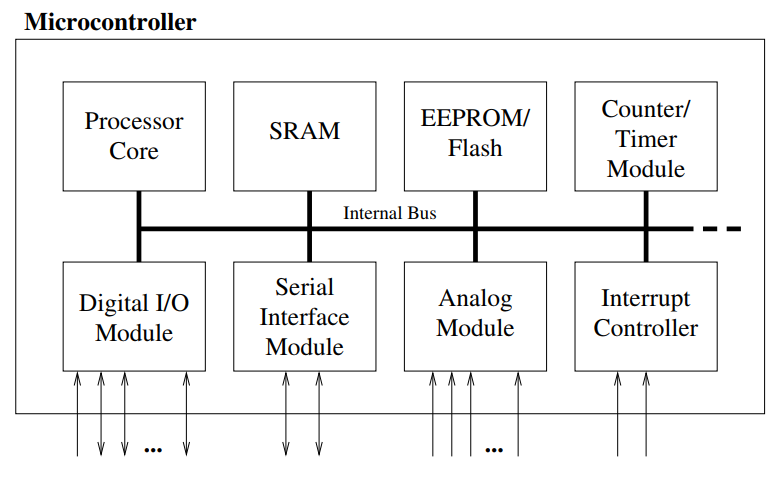
\includegraphics[scale=.5]{Capitulo2/images/microcontrolador.png}
	\caption{Diagrama de un microcontrolador básico}
	\label{fig:diagrama_dispMonitoreo}
\end{figure}
\paragraph{}
En la siguiente lista mostramos los módulos que normalmente se encuentran en un microcontrolador \citep{MarcoTeoricoMicrocontrolador}:
\begin{itemize}
	\item Procesador Core: La CPU del controlador. Contiene la unidad lógica aritmética, la unidad de control y los registros (puntero de pila, contador de programa, registro de acumulador, archivo de registro, ...).
    \item Memoria: La memoria a veces se divide en memoria de programa y memoria de datos. En los controladores más grandes, un controlador DMA maneja las transferencias de datos entre los componentes periféricos y la memoria.
    \item Controlador de interrupciones: Las interrupciones son útiles para interrumpir el flujo normal del programa en caso de (importantes) eventos externos o internos. En conjunción con los modos de sueño, ayudan a conservar energía.
    \item Temporizador o contador: La mayoría de los controladores tienen entre uno y tres temporizadores o contadores, que se pueden usar para marcar la hora de eventos, medir intervalos o contar eventos.
    \item E / S digital: Los puertos de E / S digitales paralelos son una de las características principales de los microcontroladores. La cantidad de pines de E / S varía de 3 a más de 90.
    \item E / S analógicas: Aparte de unos pocos controladores pequeños, la mayoría de los microcontroladores tienen integrado convertidores analógico - digital, que difieren en el número de canales (2-16). 
    \item Interfaces: Los controladores generalmente tienen al menos una interfaz en serie que se puede utilizar para descargar el programa y para la comunicación con la PC de desarrollo en general. Dado que las interfaces seriales también pueden usarse para comunicarse con dispositivos periféricos externos, la mayoría de los controladores ofrecen varias y variadas interfaces como SPI y SCI.
    \item Temporizador de vigilancia: Dado que los sistemas críticos para la seguridad forman un área importante de aplicación de los microcontroladores, es importante protegerse contra errores en el programa y / o el hardware. El temporizador de vigilancia se usa para reiniciar el controlador en caso de que el software se "bloquee".
    \item Unidad de depuración: Algunos controladores están equipados con hardware adicional para permitir la depuración remota del chip desde la PC. Así que no hay necesidad de descargar un software especial de depuración.
\end{itemize}

\paragraph{}
En la siguiente tabla, se muestra una comparativa entre los microcontroladores dsPIC30F3014/4013 y dsPIC30F1010/202X.


\pagebreak
\begin{longtable}{|M{2.2cm}|M{6.0cm}|M{6.0cm}|}
    \caption{Comparativa entre microcontroladores}
	% \centering
	% \begin{tabular}
	\hline
	\textbf{ Parámetro } & \textbf{Microcontrolador} & \textbf{Microcontrolador} \\ \hline
	
 	- & dsPIC30F3014/4013 & dsPIC30F1010/202X \\\hline
 	 
 	Conjunto de instrucciones  &
    84 & 83 \\ \hline
    Arquitectura   &
    Harvard & Harvard \\ \hline
    Bits en formato de instrucción  &
    24 & 24 \\ \hline
    Bits en la ruta de datos  &
    16 & 16 \\ \hline
    MIPS  &
    30 & 30 \\ \hline
    Fuentes de instrucción  &
    33 & 32 \\ \hline
    
 	 
    Características especiales del microcontrolador
    &
    -Memoria del programa Flash mejorada: 10.000 ciclos de borrado / escritura (min.) Para rango de temperatura industrial, 100k (usualmente)
    \newline-Auto-reprogramable bajo control de software
    \newline-Reinicio de encendido (POR), temporizador de encendido (PWRT) y temporizador de arranque del oscilador (OST)
    \newline-Temporizador de vigilancia flexible (WDT) con bajo en chip
    \newline-Oscilador de potencia RC para un funcionamiento confiable
    \newline-Operación de monitor de reloj a prueba de fallos
    \newline-Detecta fallas de reloj y cambia a bajo en chip oscilador de potencia RC
    \newline-Código de protección programable
    \newline-Programación Serial en Circuito (ICSP)
    \newline-Modos de gestión de energía seleccionables
    \newline-Modos Sleep, Idle y Alternate Clock
	& 
    -Memoria del programa Flash mejorada: 10.000 ciclos de borrado / escritura (min.) Para rango de temperatura industrial, 100K (usualmente)
    \newline-Memoria de datos EEPROM: 100.000 ciclos de borrado / escritura (min.) Para rango de temperatura industrial, 1M (usualmente)
    \newline-Auto-reprogramable bajo control de software
    \newline-Reinicio de encendido (POR), temporizador de encendido (PWRT) y temporizador de arranque del oscilador (OST)
    \newline-Temporizador de vigilancia flexible (WDT) 
    \newline-Detecta fallas de reloj y cambia a chip
    \newline-Oscilador RC de baja potencia
    \\ \hline

	Características periféricas  
    &
	-Hasta cinco temporizadores/contadores de 16 bits; temporizadores de 16 bits opcionalmente emparejados en módulos temporizadores de 32 bits
	\newline-Una función de entrada de captura de 16 bits
	\newline-Dos funciones de salida de comparación / PWM de 16 bits
    &
	-Tres temporizadores/contadores de 16 bits; temporizadores de 16 bits opcionalmente emparejados en módulos temporizadores de 32 bits
	\newline-Hasta cuatro funciones de entrada de captura de 16 bits
	\newline-Hasta cuatro funciones de salida de 16 bits de comparación / PWM
	\hline
	
	% \end{tabular}
	
	\label{tabla_riesgos}
\end{longtable}

\pagebreak



\section{Red de sensores}
Una red de sensores consiste en un conjunto de dispositivos denominados sensores que están conectados entre sí, para el monitoreo y sensado de condiciones físicas y/o ambientales en áreas remotas; dichos sensores pueden estar distribuidos físicamente y para referirnos a un sensor en específico como parte de la red, se le denomina nodo sensor. 
\paragraph{}
El propósito de una red de sensores es el de recolectar información de interés, es decir, la variable física sensada o monitoreada, para posteriormente transmitir dicha información con el objeto de ser procesada y analizada. 
\paragraph{}
Dado que existen una gran cantidad de dispositivos sensores implica que pueden implementarse diferentes tipos de redes de sensores de acuerdo al uso o aplicación que se le quiera dar, como por ejemplo: fenómenos meteorológicos, sistemas de emergencia o de cuidados médicos, por mencionar algunos \citep{MarcoTeorico16}.

\paragraph{Sensor}
Un sensor es un dispositivo que es capaz de transformar una señal o variable proveniente de fenómenos físicos, como pueden ser: temperatura, presión, humedad, aceleración, entre otros; en una señal de salida transducible a una señal eléctrica \citep{MarcoTeorico20} .
\paragraph{}
Existe una variedad de sensores, y pueden ser clasificados bajo diferentes criterios (principio de funcionamiento, señal de salida, rango de valores, nivel de integración, variable física de entrada).

